
\begin{refsection}
	\startcontents[chapters]	

\chapter{Regression Analysis}\label{ch:regression-analysis}
%\minitoc
	\printcontents[chapters]{}{1}{}


\section{Linear regression analysis: basics}\label{ch:theory-of-statistics:sec:linear-regression-analysis}\index{linear regression}
\begin{mdframed}
	\textbf{notations:}
	\begin{itemize}
		\item $\bm{1}$ is the vector of all 1.
		\item $J$ is a square matrix with all 1.
	\end{itemize}
\end{mdframed}


\subsection{linear regression models}
\begin{definition}[simple linear regression]
	The simple linear regression model \textbf{assumes} that a random variable $Y$ has a linear dependency on a non-random variable $X \in \R$ given as
	$$Y = \beta_0 + \beta_1 X + \epsilon$$
	where $\beta_0,\beta_1$ are unknown model parameters, and $\epsilon$ is a random variable. 
	Given the observed sample pairs $(x_1,y_1),(x_2,y_2),..., (x_n,y_n)$ as $y_i = \beta_0 + \beta_1 x_i + \epsilon_i$ and we \textbf{further make the following assumptions on $\epsilon$} as
	\begin{itemize}
		\item $E[\epsilon_i] = 0,\forall i$.
		\item $Var[\epsilon_j] = \sigma^2,\forall i$; and $\sigma^2$ is unknown.
		\item $cov(\epsilon_i,\epsilon_j) =\sigma^2 \delta_{ij},\forall i,j$.
	\end{itemize} 	
\end{definition}


\begin{definition}[multiple linear regression model]\label{ch:statistical-models:def:multipleLinearRegressionModel}
	The multiple linear regression model \textbf{assumes} that a random variable $Y$ has a linear dependency on a non-random vector $X = (X_1,X_2,...,X_{p-1}) \in \R^{p-1}$ given as
	$$Y = \beta_0 + \beta_1 X_1 +\beta_2 X_2 + ... +\beta_{p-1} X_{p-1} + \epsilon$$
	where $\beta_0,\beta_1, ...,\beta_p$ are unknown model parameters, and $\epsilon$ is a random variable. 
	Given the observed sample pairs $(x_1,y_1),(x_2,y_2),..., (x_n,y_n), x\in \R^{p-1}, y\in \R$ as $y_i = \beta_0 + \beta_1 x_{i1} + \beta_2 x_{i2} + ... + \epsilon_i$ and we \textbf{further make the following assumptions on $\epsilon$} as
	\begin{itemize}
		\item $E[\epsilon_i] = 0,\forall i$
		\item $cov(\epsilon_i,\epsilon_j) = \sigma^2\delta_{ij}$ and $\sigma^2$ is unknown.
	\end{itemize} 	
\end{definition}

\begin{assumption}[standard assumptions of linear regression model]\label{ch:regression-analysis:assumption:LinearRegressionStandardAssumption} \cite[17]{greene2017econometric}
The standard assumption of a linear regression model consists of
\begin{description}
	\item[A1. Linear model assumption] The random variable $Y$ has a linear dependency on $X$ give by
	$$Y = \beta_0 + \beta_1 X_1 +\beta_2 X_2 + ... +\beta_{p-1} X_{p-1} + \epsilon.$$
	\item[A2. Linear independence of regressors] There is no linear dependency exists among regressors $X_1, X_2,...,X_{p-1}$.  
	\item[A3. Indepedence between regressor and noise] The regressors $(X_1,X_2,...,X_{p-1})$ are independent of the noise term $\epsilon$.
	\item[A4. Homoscedaticity] Homoscendaticity refers to that the conditional variance $Var[\epsilon|X_i],i=1,...,p-1$ is a constant given the observation of the regressors. This can be written by
	$$ Var[\epsilon | X_i] = \sigma^2, \forall i.$$  
	\item[A5. Data generation of regressors] The regressor data $(x_1,x_2,...)$ can be either constants from experimental design or realizations of random variables. 
	\item[A6. Normal distribution of noise] The noise random samples $\epsilon_1, \epsilon_2,...$ have normal distribution and independent of each other, which can be written by
	$$\epsilon | X_i \sim N(0, \sigma^2 I), \forall i.$$ 
\end{description}	
\end{assumption}

\begin{table}[H]
	\begin{tabular}{|l|l|}
		\hline
		With non-random $x$                              & With random $x$                                      \\ \hline
		A1: $y = \beta_1 + x^T\beta_2+e$, with $x$ fixed & A1: $y = \beta_1 + x^T\beta_2+e$, with $x, e$ random \\ \hline
		A2: $E[e] = 0$                                   & A2: $E[e] = 0$                                       \\ \hline
		A3: $Var[e] = \sigma^2$                          & A3: $Var[e] = \sigma^2$                              \\ \hline
		A4: $Cov(e_i, e_j) = 0$                          & A4: $Cov(e_i, e_j) = 0$                              \\ \hline
		A5: $x$                                          & A5: $x$                                              \\ \hline
		A6: $e$ is normal                                & A6: $e$ is normal                                    \\ \hline
	\end{tabular}
\end{table}

\begin{remark}[understand data generation process]\cite[25]{greene2017econometric}
In the application of linear regression model, there are usually two types of data generation processses on how we obtain the regressor observations.	
\begin{itemize}
	\item In a physics experiment, the experimentalist will choose different regressor values and observe the output $y$. In this case, regressor values are certainly not sampled from a distribution.
	\item In a social study where social scientist usually cannot design experiments like physicist. In this case, we assume regressors are random variables and regressor observations are sampled from a distribution.  
\end{itemize}
\end{remark}


\begin{note}[understand linear regression from the perspective of approximation]\hfill
\begin{itemize}
	\item In the linear regression model, our ultimate goal is to model the \textbf{conditional distribution} of random variable $Y$ given by the observations of random variables $X_1,X_2,...,X_p$, that is
	$$P(Y|X_1,X_2,...,X_p).$$
	\item  We know that the distribution $P(Y|X_1,X_2,...,X_p)$ is fully determined by all of its moments given by
	\begin{align*}
	&E[Y|X_1,X_2,...,X_p] \\
	&E[Y^2|X_1,X_2,...,X_p] \\
	&E[Y^3|X_1,X_2,...,X_p] \\
	&\cdots
	\end{align*} 
	\item In the linear model, we \textbf{assume} 
	$$Y = \beta_0 + \beta_1 X_1 +\beta_2 X_2 + ... +\beta_{p} X_p + \epsilon, \epsilon \in N(0,\sigma^2).$$
	In this way, the conditional distribution $P(Y|X_1,...,X_p)$ is fully determined by the vector $\beta$ and the variance coefficent $\sigma^2$. 
	In particular
	\begin{itemize}
		\item the first moment
	$$E[Y|X_1,...,X_p] = f(X_1,...,X_p)=\beta_0 + \beta_1 X_1 +\beta_2 X_2 + ... +\beta_{p} X_p.$$ 
	\item the second moment(variance)
	$$Var[Y|X_1,...,X_p] = g(X_1,...,X_p) = \sigma^2.$$ 
		By assuming $E[\epsilon_i\epsilon_j]=\sigma^2\delta_{ij}$ we are assuming $Var[Y|X_1,X_2,...,X_p]$ is homogeneous, i.e., has no dependence on $X_1,X_2,...,X_p$
	\end{itemize} 
	\item In our linear model, we select coefficients $\beta$ to maximize the likelihood of observation $y_1,y_2,...,y_n$ given observations of $X_1,...,X_p$.
\end{itemize}	
\end{note}



\subsection{Least square solutions}
\subsubsection{Orthogonal projection and the least square result}
\begin{lemma}[essential properties of orthogonal projection]\label{ch:theory-of-statistics:th:propertylinearregression}\index{orthogonal projection}
	Let $X$ be a matrix of size $n\times p$. 
	Define $$H = X(X^TX)^{-1}X^T,$$ we have
	\begin{itemize}
		\item $(X^TX)^{-1}$ exists if $X$ has full column rank.
		\item $rank((X^TX)) = p$, $rank(H) = p$ and $rank(I-H) = n-p$.
		\item $H$ is symmetric and idempotent; in other words, $H$ is an orthogonal projector onto the subspace spanned by columns of $X$.
		\item $I-H$ is symmetric and idempotent; in other words, $I-H$ is an orthogonal projector onto the orthogonal complementary subspace spanned by columns of $X$.
		\item The prediction is given as $HY$
		\item The residual is given as $(I-H)Y$
	\end{itemize}
\end{lemma}
\begin{proof}
	(1) Use the fact that $\cN(X^TX) = \cN(X)$(\autoref{ch:linearalgebra:ranklemmaone}). If $X$ is invertible then $X^TX$ is invertible.
	(2) $X^TX$ is invertible, therefore has full rank of $p$.  Use \autoref{ch:linearalgebra:th:rankOfMatrixProducts}. $$rank(X(X^TX)^{-1}) = rank((X^TX)^{-1}) = p, rank(X(X^TX)^{-1}X^T) = rank((X^TX)^{-1}) = p.$$
	(3) Direct verification. \autoref{ch:linearalgebra:th:characterizationoforthogonalprojector}.
	(4) $(I-H)^T = I - H$, and $(I-H)(I-H) = (I - 2H + H^2) = (I - 2H + H) = I - H$.
	(5) $\hat{Y} = X(X^TX)^{-1}X^TY = HY$.
	(6) $\epsilon = Y - \hat{Y} = Y - HY = (I-H)Y$.
\end{proof}


\begin{remark}[change of coefficient value after adding or omitting regressors]
Consider a original linear regression model	given by
$$Y = \beta_0 + \beta_1 X_1 + \cdots + \beta_{k-1} X_{k-1}. $$
Suppose now we add a new regressor $X_k$. Then the coefficient $\hat{\beta}_k$ has the following change after adding the new regressor
\begin{itemize}
	\item If $X_{k}$ is demeaned and uncorrelated with $X_1,X_2,...,X_{k-1}$, then the coefficient $\hat{\beta}_i$ will not change.
	\item If $X_{k}$ has finite mean and uncorrelated with $X_1,X_2,...,X_{k-1}$, then the coefficient $\hat{\beta}_i, i=1,2,...,k-t$ will not change, coefficient $\hat{\beta}_0$ will decrease if $X_k$ is positively correlated with $Y$ and has positive mean (i.e., positively correlated with unit vector $\bm{1}$), and coefficient $\hat{\beta}_0$ will increase if $X_k$ is positively correlated with $Y$ and has negative mean (i.e., negatively correlated with unit vector $\bm{1}$). A simple intuition is
	$$\beta_0 = E[Y] - \beta_1E[X_1] - \cdots - \beta_{k}E[X_k].$$
	\item More generally, if $X_{k}$ is arbitrary, then the coefficient $\hat{\beta}_i$ will decrease if $Corr(X_k,Y)$ and $Corr(X_k,X_i)$ have the same sign (competing effect) and the coefficient $\hat{\beta}_i$ will increase if $Corr(X_k,Y)$ and $Corr(X_k,X_i)$ have the opposite (compensating effect). For example, suppose $Corr(X_k,Y) > 0$, then $\hat{\beta}_k > 0$. Because $Corr(X_k,X_i) < 0$, $\hat{\beta}_i$ needs to increase to compensate the offsetting effects due to $X_k$.
\end{itemize}
\end{remark}


\begin{theorem}[least square solution: general case ]\label{ch:statistical-models:th:leastSquareSolution}\label{ch:statistical-models:th:OrdinaryLinearRegressionleastSquareSolution}\index{least square}
	The multiple linear regression with n samples can be written as
	\begin{align*}
	\begin{bmatrix}
	y_1\\
	y_2\\
	\vdots\\
	y_n
	\end{bmatrix} = \begin{bmatrix}
	1 & x_{11} & x_{12} & \dots & x_{1(p-1)}\\
	1 & x_{21} & x_{22} & \dots & x_{2(p-1)}\\
	\vdots & \vdots & \vdots & \vdots & \vdots \\
	1 & x_{n1} & x_{n2} & \dots & x_{n(p-1)}\\
	\end{bmatrix}
	\begin{bmatrix}
	\beta_0\\
	\beta_1\\
	\vdots\\
	\beta_{p-1}
	\end{bmatrix}
	+ \begin{bmatrix}
	\epsilon_1\\
	\epsilon_2\\
	\vdots\\
	\epsilon_{n}
	\end{bmatrix}
	\end{align*}
	with matrix form
	$$Y = X\beta + \epsilon.$$
Assume the standard assumptions (\autoref{ch:regression-analysis:assumption:LinearRegressionStandardAssumption}) hold.	
	The \textbf{unique minimizer} to the problem 
	$$\min_\beta (Y-X\beta)^T(Y - X\beta)$$
	is given as
	$$\hat{\beta} = (X^TX)^{-1}X^TY,$$
	in particular, $$\hat{\beta}_0 = \mean{y} - \sum_{i=1}^{p-1} \hat{\beta}_i \mean{x}_i$$
	$$\hat{y}_i - \mean{y} =\sum_{i=1}^{p-1} \hat{\beta}_j (x_{ij}-\mean{x}_j) $$
	Moreover, we have
	\begin{itemize}
		\item $E[\hat{\beta}] = \beta$.
		\item If $Cov[Y] = \sigma^2I$, then $Cov[\hat{\beta}] = \sigma^2(X^TX)^{-1}$.($\hat{\beta}$ is not necessarily normal).
		\item To get each individual coefficient, we have 
		$$\hat{\beta}_i = \frac{X_i^T(I - H_{-i})Y}{X_i^T(I-H_{-i})X_i},$$
		where $H_{-i} = X_{-i}(X_{-i}^TX_{-i})^{-1} X_{-i}^T$, $X_{-i}$ is the matrix without column $i$.
	\end{itemize}
\end{theorem}
\begin{proof}
	See \autoref{ch:functional-analysis:th:normalequation}.\\
	(1) (unbiasedness) $E[\hat{\beta}] = (X^TX)^{-1}X^T E[Y] = (X^TX)^{-1}X^TX\beta = \beta.$
	(2) (variance) $Cov[\beta] = (X^TX)^{-1}X^TCov[Y]((X^TX)^{-1}X^T)^T = \sigma^2(X^TX)^{-1}$.
	(3) See \autoref{ch:functional-analysis:th:normalequation}. We can interpret as first projecting $Y$ into the null space of $(I-H_{-i})X_{-i}$ and project onto $X_i$. 
\end{proof}

\begin{theorem}[least square solution: demean case ]\index{least square}\label{ch:statistical-models:th:leastSquareSolutionDemeanCase}
Consider a multiple linear regression problem where $y$ and $x$ are demeaned; that is, $\sum_i y_i = 0, \sum_{i}x_{i,j} = 0, j=1,2,...,p$. 	The multiple linear regression with n samples can be written as
\begin{align*}
\begin{bmatrix}
y_1\\
y_2\\
\vdots\\
y_n
\end{bmatrix} = \begin{bmatrix}
\beta_0\\
\beta_0\\
\vdots\\
\beta_0
\end{bmatrix}+\begin{bmatrix}
x_{11} & x_{12} & \dots & x_{1(p)}\\
x_{21} & x_{22} & \dots & x_{2(p)}\\
\vdots & \vdots & \vdots & \vdots \\
x_{n1} & x_{n2} & \dots & x_{n(p)}\\
\end{bmatrix}
\begin{bmatrix}
\beta_0\\
\beta_1\\
\vdots\\
\beta_{p}
\end{bmatrix}
+ \begin{bmatrix}
\epsilon_1\\
\epsilon_2\\
\vdots\\
\epsilon_{n}
\end{bmatrix}.
\end{align*}
	with matrix form
	$$Y = \beta_0\bm{1} + X\beta + \epsilon$$
	The \textbf{unique minimizer} to the problem 
	$$\min_\beta (Y-\beta_0\bm{1} -X\beta)^T(Y - \beta_0\bm{1} - X\beta)$$
	is given as
	$$\hat{\beta}_0 = \mean{y} - \sum_{i=1}^{p-1} \hat{\beta}_i \mean{x}_i,$$
	and
	$$\hat{\beta} = (\tilde{X}^T\tilde{X})^{-1}\tilde{X}^T\tilde{Y},$$
	where $\tilde{X}_{ij} = X_{ij} - \mean{x}_j, \tilde{Y} = Y - \mean{y}.$
	
	Eventually, we can write
	$$\hat{y}_i - \mean{y} =\sum_{j=1}^{p-1} \hat{\beta}_j (x_{ij}-\mean{x}_j) $$
	Moreover, we have
	\begin{itemize}
		\item $E[\beta_0] = \beta_0, E[\hat{\beta}] = \beta$.
		\item (to do)If $Cov[Y] = \sigma^2I$, then $Cov[\hat{\beta}] = \sigma^2(X^TX)^{-1}$.($\hat{\beta}$ is not necessarily normal)
	\end{itemize}
\end{theorem}
\begin{proof}
(1)We can use the projection theorem \autoref{ch:functional-analysis:th:normalequation} or use the following optimization method. 

$$\min f = (Y - \beta_0\bm{1} - X\beta)^T(Y - \beta_0\bm{1} - X\beta)$$
over $\beta_0, \beta_1$, we have
\begin{align*}
f(\beta_0,\beta_1) &= Y^TY + n^2\beta_0^2 + (\beta^TX^TX\beta)+ 2n\beta_0\bm{1}^TX\beta - 2n\beta_0\bm{1}^TY- 2Y^TX\beta \\
&= Y^TY + n^2\beta_0^2 + (\beta^TX^TX\beta)+ 2n\beta_0\bm{1}^TX\beta - 2n\beta_0\sum_{i=1}^n y_i - 2Y^TX\beta 
\end{align*} 
The first order condition on $\beta_0$ gives that
$$\beta_0 = \frac{1}{n}\sum_{i=1}^n y_i - \frac{1}{n} \bm{1}^TX\beta;$$
Plug in $\beta_0$(note that $(I - \frac{1}{n}\bm{1}\bm{1}^T)X = \tilde{X}$), we can transform the minimization problem to
$$f(\beta_0,\beta_1) = (\tilde{Y} - \tilde{X}\beta)^T(\tilde{Y} - \tilde{X}\beta).$$
Then we can use the results in the general case(\autoref{ch:statistical-models:th:leastSquareSolution}) to obtain the estimator for $\beta$.
	(2) (unbiasedness) 
	\begin{align*}
	E[\hat{\beta}_0] &= E[ \mean{y} - \sum_{i=1}^{p-1} \hat{\beta}_i \mean{x}_i] \\
	&= E[ \mean{y}] - \sum_{i=1}^{p-1} E[\hat{\beta}_i \mean{x}_i] \\
	&= E[\frac{1}{n}\bm{1}^TY] - \sum_{i=1}^{p-1} E[\hat{\beta}_i ]\mean{x}_i \\
	&= \frac{1}{n}\bm{1}^TE[Y] - \sum_{i=1}^{p-1} \frac{1}{n}\bm{1}X_i\beta_i\\
	&=\frac{1}{n}\bm{1}^T(Y - X\beta)\\
	&=\frac{1}{n}\bm{1}^T(\beta_0\bm{1} + X\beta + \epsilon - X\beta)\\
	& = \frac{1}{n}\bm{1}^T\beta_0\bm{1} \\
	&=\beta_0.
	\end{align*}
where we use the fact that $E[\hat{\beta}] = \beta$ proved later.
	
	$$E[\hat{\beta}] = (\tilde{X}^T\tilde{X})^{-1}\tilde{X}^T E[Y] = (X^TX)^{-1}\tilde{X}^T\tilde{X}\beta = \beta.$$
\end{proof}

\begin{remark}[another way to see the coefficients in the demean case]
From \autoref{ch:statistical-models:th:leastSquareSolution}, we can see that if we want to get the coefficients $\beta = (\beta_1,\beta_2,...,\beta_{p-1})$, we can use
$$\beta = (X^T(I-H_{0})(I-H_{0})X)^{-1}X^T(I - H_{0})(I - H_{0})Y,$$
where $H_{0} = \frac{1}{n}\bm{1}\bm{1}^T$.
Note that $(I - H_{0})Y$ will generate a demeaned $Y$ and $(I - H_{0})X$ will generate a column-wise demeaned $X$. This is because the $I - H_0$ operator will is a demean operator.
\end{remark}



\begin{corollary}[special cases, least square solution for simple regression]\label{ch:regression-analysis:th:leastSquareSolutionSimpleLinearRegression}
Define
$$S_{XX} = \sum_i (x_{i}-\mean{x})^2, S_{XY} =  \sum_i (x_{i}-\mean{x})(y_i - \mean{y}, S_{YY} = \sum_i (y_{i}-\mean{y})^2,$$
and
$$S_{X} = \sqrt{S_{XX}}, S_Y = \sqrt{S_{YY}}.$$

It follows that
	\begin{itemize}
		\item For the zero order model $y = \beta_0 + \epsilon$, $$\hat{\beta}_0 = \frac{\ip{y,\bm{1}}}{\ip{\bm{1},\bm{1}}} = \frac{1}{n}\sum_i y_i$$
		\item For the first order model $y = \beta_0 +\beta_1 x+ \epsilon$, $$\hat{\beta} = [X^TX]^{-1}X^TY$$
		we have $$\hat{\beta}_0 = \mean{y} - \hat{\beta}_1\mean{x}$$ and
		\begin{align*}
		\hat{\beta}_1 &= \frac{\sum_i (x_{i}-\mean{x})(y_i - \mean{y})}{\sum_i (x_{i}-\mean{x})^2} \\
		& = \frac{S_{XY}}{S_{XX}} \\
		& = \frac{\sum_i (x_{i}-\mean{x})y_i }{\sum_i (x_{i}-\mean{x})(x_i)} \\
		& = \frac{\sum_i x_{i}(y_i - \mean{y})}{\sum_i (x_{i}-\mean{x})x_i} \\
		& = \hat{\rho} \frac{S_Y}{S_X}
		\end{align*}
	where $\hat{\rho} = S_{XY}/S_XS_Y$ is the sample correlation coefficient between $X$ and $Y$.	
		In summary, $$\hat{y}_i = \mean{y} + \hat{\beta}_1(x_i - \mean{x}).$$
		\item In the first order model, we have conditional mean and  unconditional variance of $y$ given by
		$$E[y|x] = \beta_0+\beta_1x, Var[y] = \sigma^2, Var[\mean{y}]=\frac{\sigma^2}{n}.$$
		\item In the first order model, we have unbiased coefficient estimator
		$$E[\hat{\beta}_1] = \beta_1, E[\beta_0] = \beta_0.$$
		\item In the first order model, we have 
		$$Var[\hat{\beta}_1] = \frac{\sigma^2}{S_{XX}}, Var[\hat{\beta}_0] = \sigma^2(\frac{1}{n} + \frac{\mean{x}^2}{S_{XX}}),Cov(\hat{\beta}_1,\hat{\beta}_0) = -\frac{\sigma^2\mean{x}}{S_{XX}}$$
		where
		$$S_{XX} = \sum_i (x_{i}-\mean{x})^2=\sum_i (x_{i}-\mean{x})x_i.$$
	\end{itemize}
\end{corollary}
\begin{proof}
(2)
$$Var[y] = E[(y-E[y])^2] = E[(y-E[y|x])^2] = E[\epsilon^2] = \sigma^2.$$	
(3)Note that 
\begin{align*}
\sum_i (x_{i}-\mean{x})^2 &= x^T(I-\frac{1}{n}J)(I-\frac{1}{n}J)x \\
&= x^T(I-\frac{1}{n}J)x \\
&= x^T(x-\mean{x}\bm{1}) 
\end{align*}
and
\begin{align*}
\sum_i (x_{i}-\mean{x})(y_i - \mean{y}) &= x^T(I-\frac{1}{n}J)(I-\frac{1}{n}J)y \\
&= x^T(I-\frac{1}{n}J)y \\
&= x^T(y-\mean{y}\bm{1}) \\ 
&= y^T(x-\mean{x}\bm{1})
\end{align*}
(4)
\begin{align*}
E[\hat{\beta}_1] &= E[\frac{\sum_i (x_{i}-\mean{x})y_i }{\sum_i (x_{i}-\mean{x})(x_i)}] \\
&= E[\frac{\sum_i (x_{i}-\mean{x})(\beta_0+\beta_1x_i+\epsilon_i)}{\sum_i (x_{i}-\mean{x})(x_i)}] \\
&=\frac{\sum_i (x_{i}-\mean{x})(\beta_0+\beta_1x_i)}{\sum_i (x_{i}-\mean{x})(x_i)} \\
&=\frac{\sum_i (x_{i}-\mean{x})(\beta_0)}{\sum_i (x_{i}-\mean{x})(x_i)} + \frac{\sum_i (x_{i}-\mean{x})(\beta_1x_i)}{\sum_i (x_{i}-\mean{x})(x_i)} \\
&= 0 + \beta_1 = \beta_1.
\end{align*}
and
\begin{align*}
E[\hat{\beta}_0] &= E[\mean{y} - \hat{\beta}_1\mean{x}] \\
 &= \frac{1}{n}\sum_i E[y_i - \hat{\beta}_1x_i] \\
 &=\frac{1}{n}\sum_i E[\beta_0 + \beta_1x_i - \hat{\beta}_1x_i] \\
 &=\frac{1}{n}\sum_i \beta_0 \\
 &=\beta_0. 
\end{align*}
(5)
\begin{align*}
Var[\hat{\beta}_1] &= Var[\frac{\sum_i (x_{i}-\mean{x})y_i }{\sum_i (x_{i}-\mean{x})^2}] \\
&= Var[\frac{\sum_i (x_{i}-\mean{x})(\beta_0+\beta_1x_i+\epsilon_i)}{\sum_i (x_{i}-\mean{x})^2}] \\
&= Var[\frac{\sum_i (x_{i}-\mean{x})(\epsilon_i)}{\sum_i (x_{i}-\mean{x})(x_i)}] \\
&=\sigma^2 \sum_i \frac{\sum_i (x_{i}-\mean{x})^2}{(\sum_i (x_{i}-\mean{x})^2)^2}\\
&=\sigma^2 \frac{1}{(\sum_i (x_{i}-\mean{x})^2)}
\end{align*}
and
\begin{align*}
Var[\hat{\beta}_0] &= Var[\mean{y} - \hat{\beta}_1\mean{x}] \\
&=Var[\mean{y}] + \mean{x}^2Var[\hat{\beta}_1] -2\mean{x}Cov(\mean{y},\hat{\beta}_1)\\
&= \frac{1}{n}\sigma^2 + \mean{x}^2\sigma^2/S_{XX} + 0 \\
&=\sigma^2(\frac{1}{n} + \frac{\mean{x}^2}{S_{XX}})
\end{align*}
where $Cov(\mean{y},\hat{\beta}_1) = 0$ since
\begin{align*}
Cov(\mean{y},\hat{\beta}_1) & = E[\frac{1}{n}\sum_{i} \epsilon_i (\sum_{i}c_i\epsilon_i -\beta_1)] \\
&=\frac{1}{n}E[\sum_i c_i \epsilon_i^2] \\
&=\frac{1}{n}\sum_i c_i \sigma^2\\
&=0
\end{align*}
where 
$$c_i =\frac{ (x_{i}-\mean{x})}{\sum_i (x_{i}-\mean{x})(x_i)}, \sum_i c_i = 0.$$

To calculate $Cov(\hat{\beta}_1,\hat{\beta}_0)$, we use the fact that
\begin{align*}
\hat{\beta}_0 &= \mean{y} - \hat{\beta}_1\mean{x} \\
\hat{\beta}_0 + \hat{\beta}_1\mean{x} &= \mean{y}  \\
Var[\hat{\beta}_0 + \hat{\beta}_1\mean{x}] &= Var[\mean{y}] = \frac{\sigma^2}{n} \\
Var[\hat{\beta}_0] + Var[\hat{\beta}_1]\mean{x}^2 + 2\mean{x}Cov(\hat{\beta}_1,\hat{\beta}_0) &= \frac{\sigma^2}{n} 
\end{align*}
then we can get 
$$Cov(\hat{\beta}_1,\hat{\beta}_0) = -\frac{\sigma^2\mean{x}}{S_{XX}}.$$
\end{proof}

\begin{remark}[interpretation]\hfill
\begin{itemize}
	\item We can interpret $x_i-\mean{x}$ and $y_i-\mean{y}$ as the part remove the projection (that is, $\mean{x}\bm{1}, \mean{y}\bm{1}$)onto the constant value subspace of $\bm{1}$. To see this, we have
	$$\sum_{i=1}^{n}(x_i - \mean{x})\mean{x} = n\mean{x}^2-n\mean{x}^2 = 0,$$
	and
		$$\sum_{i=1}^{n}(y_i - \mean{y})\mean{y} = n\mean{y}^2-n\mean{y}^2 = 0.$$
	Therefore, the formula 
	$$\hat{\beta}_1 = \frac{\sum_i (x_{i}-\mean{x})(y_i - \mean{y})}{\sum_i (x_{i}-\mean{x})^2}$$
	is consistent with the formula
	$$\hat{\beta}_i = \frac{X_i^T(I - H_{-i})Y}{X_i^T(I-H_{-i})X_i},$$
	where $H_{-i} = X_{-i}(X_{-i}^TX_{-i})^{-1} X_{-i}^T$, $X_{-i}$ is the matrix without column $i$.
	\item The coefficient $\hat{\beta}_j$ represents the additional contribution from $X_j$ after accounting for the contribution from $\bm{1},X_1,...,X_{j-1}, X_{j+1},...,X_p$.
\end{itemize}	

\end{remark}

\subsubsection{Orthogonal input and successive regression}


\begin{theorem}[multiple linear regression with orthogonal input]
Consider a multiple linear regression problem  with n samples can be written as
\begin{align*}
\begin{bmatrix}
y_1\\
y_2\\
\vdots\\
y_n
\end{bmatrix} = \begin{bmatrix}
\beta_0\\
\beta_0\\
\vdots\\
\beta_0
\end{bmatrix}+\begin{bmatrix}
1 & x_{11} & x_{12} & \dots & x_{1(p-1)}\\
1 & x_{21} & x_{22} & \dots & x_{2(p-1)}\\
\vdots & \vdots & \vdots & \vdots & \vdots \\
1 & x_{n1} & x_{n2} & \dots & x_{n(p-1)}\\
\end{bmatrix}
\begin{bmatrix}
\beta_0\\
\beta_1\\
\vdots\\
\beta_{p-1}
\end{bmatrix}
+ \begin{bmatrix}
\epsilon_1\\
\epsilon_2\\
\vdots\\
\epsilon_{n}
\end{bmatrix}.
\end{align*}
with matrix form
$Y = X\beta + \epsilon$.

\textbf{Further assume columns of $X$ are orthogonal.}\footnote{Note that orthogonality implies $y$ and $x$ are demeaned; that is, $\ip{\bm{1},y} = 0\implies\sum_i y_i = 0, \sum_{i}x_{i,j} = 0, j=1,2,...,p$.} 
Then 
\begin{itemize}
	\item we have 
	$$\hat{\beta}_i = \frac{ \ip{X_i,Y}}{\ip{X_i,X_i}},$$
	where $X_i$ is the column $i$ of $X$ and $\ip{\cdot, \cdot}$ is inner product.
	\item Further adding or omitting \textbf{another orthogonal regressor} will not affect other already-determined $\hat{\beta}_i$.
\end{itemize}
\end{theorem}
\begin{proof}
From OLS solution (\autoref{ch:statistical-models:th:OrdinaryLinearRegressionleastSquareSolution}), we have
$$\hat{\beta} = (X^TX)^{-1}X^TY.$$
Under the orthogonality assumption, $X^TX$ will be a diagonal matrix such that the component of $\hat{\beta}$ can be written by
$$\hat{\beta}_i = \frac{ \ip{X_i,Y}}{\ip{X_i,X_i}}.$$
After incorporating new orthogonal regressors, the $\hat{\beta}_i$ remain the same.

\end{proof}	


\begin{remark}[orthogonalization for linear regression]
We can use QR decomposition to make the input orthogonal to each other; such idea gives the following successive regression method.
\end{remark}



\begin{method}[successive regression method]
Consider a multiple linear regression problem consisting of column input vectors $X_1,...,X_p$ and output vector $Y$.	
\begin{itemize}
	\item Initialize $Z_0 = 1$.
	\item Regress $X_1$ on $Z_0$, and denote $Z_1$ as the residual vector,
	$$Z_1 = X_1 - \frac{\ip{X_1,Z_0}}{\ip{Z_0,Z_0}}Z_0.$$
	\item Similarly, regress $X_i$ on $Z_0,Z_1,...,Z_{i-1}$ for $i=2,...,p$, and denote $Z_i$ as the residual vector,
	$$Z_i = X_i - \sum_{j=0}^{i-1}\frac{\ip{X_1,Z_j}}{\ip{Z_j,Z_j}}Z_j.$$
	
	\item Since $Z_0,Z_1,...,Z_p$ are orthogonal, then 
	$$\hat{\beta}_i =  \frac{ \ip{Z_i,Y}}{\ip{Z_i,Z_i}}.$$
\end{itemize}
\end{method}


\subsubsection{Frisch-Waugh-Lovell(FWL) theorem and partial regression}


\begin{theorem}[Frisch-Waugh-Lovell theorem]\index{Frisch-Waugh-Lovell theorem}\label{ch:regression-analysis:th:LinearRegressionPartialRegressionFrisch-Waugh-LovellTheorem}
Consider a linear regression formulation with standard assumptions
$$Y = X_1\beta_1 + X_2\beta_2 + \epsilon,$$
where $Y\in \R^N, X_1\in \R^{N\times k_1}, X_2\in \R^{N\times k_2}, \beta_1\in\R^{k_1}, \beta_2\in \R^{k_2}$. We assume $X_1,X_2$ matrices have full column rank. Let $\hat{\beta}_1,\hat{\beta}_2$ be the least square estimators.
It follows that
\begin{itemize}
	\item $$\hat{\beta}_2 = (X_2^TM_1X_2)^{-1}X_2M_1Y,$$
	where $M_1 = I - H_1, H_1 = X_1(X_1^TX_1)^{-1}X_1^T$.
	\item The estimator $\hat{\beta}_2$ can be viewed as the least square estimator from a modified linear regression problem given by
	$$M_1Y = M_1X_2 \beta + M_1\epsilon.$$
	\item $$Var[\hat{\beta}_2] = \sigma^2 (X_2^TM_1X_2)^{-1}. $$
\end{itemize}	
\end{theorem}
\begin{proof}

(2) If we multiply the null orthogonal projector $M_1$ to both sides of 
$$Y = X_1\beta_1 + X_2\beta_2 + \epsilon$$
and get
$$M_1Y = M1X_2 \beta + M_1\epsilon.$$

Alternatively, directly apply least square solution to $M_1Y = M1X_2 \beta + M_1\epsilon$ we also get
\begin{align*}
\hat{\beta}_2 &= (X_2^TM_1^TM_1X_2)^{-1}X_2^TM_1^TM_1Y \\
			  &= (X_2^TM_1X_2)^{-1}X_2^TM_1Y
\end{align*}
where we use $M_1^T = M_1, M^T_1M_1 = M_1.$
(3)
\begin{align*}
Var{\beta}_2 &= (X_2^TM_1X_2)^{-1}X_2^TM_1Var[Y] ((X_2^TM_1X_2)^{-1}X_2^TM_1Y)^T \\
			 &= (X_2^TM_1X_2)^{-1}X_2^TM_1\sigma^2 I ((X_2^TM_1X_2)^{-1}X_2^TM_1Y)^T \\
			 &= \sigma^2 (X_2^TM_1X_2)^{-1}.
\end{align*}
\end{proof}



\subsubsection{Gauss-Markov theorem}



\begin{theorem}[Gauss-Markov theorem, best linear unbiased estimator]\label{ch:regression-analysis:th:BestLinearUnbiasedEstimator}
	Given the statistical model
	$$Y= X\beta + \epsilon, E[\epsilon] = 0, Cov(\epsilon) = \sigma^2 I$$
	with $\beta$ being the model parameter, $y$ being the observations, the \textbf{uniformly minimum variance estimators among all linear unbiased estimators} is given by
	$$\hat{\beta} = (X^TX)^{-1}X^TY.$$
	
	As a summary, we have
	\begin{itemize}
		\item $E[\hat{\beta}] = \beta$.
		\item $Cov[\hat{\beta}] = \sigma^2(X^TX)^{-1}$.
		\item Furthermore, if $\epsilon$ is Gaussian noise, i.e., $\epsilon \sim MN(0, \sigma^2 I)$, and $Y,X_1,X_2,...,X_n$ are multivariate Gaussian, then $\hat{\beta}$ is the uniformly minimum variance estimator among all estimators.
	\end{itemize}
\end{theorem}
\begin{proof}
	
	(1) (unbiasedness) $E[\beta] = (X^TX)^{-1}X^T E[Y] = (X^TX)^{-1}X^TX\beta = \beta.$
	(2) Let $\theta' = AY $ be any other unbiased linear estimator, and assume $\theta' = (X^TX)^{-1}X^T + D $ for some matrix $D$. The unbiasedness requires that $$E\theta' = \theta(I + DX) = \theta \Rightarrow DX = 0.$$
	The variance of the estimator is given as
	\begin{align*}
	E[(\theta' - \theta)(\theta' - \theta)^T] &= E[(D + (X^TX)^{-1}X^T)\epsilon\epsilon^T(D+(X^TX)^{-1}X^T)^T]\\
	&=DE[\epsilon\epsilon^T]D^T + (X^TX)^{-1} \sigma^2 I \\
	&=\sigma^2 (DD^T + (X^TX)^{-1}) = \sigma^2 DD^T + Var(\theta) \geq Var(\theta).
	\end{align*} 
	Here the $\geq$ sign is in the semi-positive matrix sense.  
	(3) Note that the joint pdf of $y= (y_1,...,y_n)$ can be written by
$$f(y;\beta, \sigma^2) = \prod_{i=1}^{N} N(y_i;x_i,\beta, \sigma^2) = (2\pi\sigma^2)^{-N/2}\exp(-\frac{1}{2\sigma^2}(y_i-x_i^T\beta)^T(y_i-x_i^T\beta)).$$

The Fisher information assoiciated with $f$ is given by
\begin{align*}
\frac{\Pa \log f}{\Pa \beta} &= \frac{1}{\sigma^2}(Y-X\beta)^TX. \\
I(\beta) &= -E[\frac{\Pa^2 \log f}{\Pa \beta\Pa \beta^T}] = \frac{1}{\sigma^2}X^TX.
\end{align*}
It is clear that $Cov[\hat{\beta}] = [I(\beta)]^{-1}$; that is, the variance of $\hat{\beta}$ reaches the Cramer-Rao lower bound (\autoref{ch:theory-of-statistics:th:CramerRaoLowerBoundMultivariateEstimation}). Therefore, $\hat{\beta}$ has the uniformly minimum variance. 
\end{proof}


\begin{corollary}[maximum likelihood estimation of parameters in simple linear regression]
The likelihood function for the multiple linear regression problem is given by	
$$L(\beta_0,\beta_1, \sigma^2) = \prod_{i=1}^{N} N(y_i;x_i,\beta_0,\beta_1, \sigma^2) = (2\pi\sigma^2)^{-N/2}\exp(-\frac{1}{2\sigma^2}\sum_{i=1}^{N}(y_i-\beta_0-\beta_1x_i)^2),$$
and the logarithm of this function is
$$l(\beta_0,\beta_1, \sigma^2) = -\frac{N}{2}\ln(2\pi)-\frac{N}{2}\ln(\sigma^2) -\frac{1}{2\sigma^2}\sum_{i=1}^{N}(y_i-\beta_0-\beta_1x_i)^2.$$

We have the following derivatives
\begin{itemize}
	\item 
	$$\frac{\Pa l}{\Pa \beta_1} = -2\sum_{i=1}^{N}(y_i-\beta_0-\beta_1x_i)x_i.$$
	\item
	$$\frac{\Pa l}{\Pa \beta_0} = -2\sum_{i=1}^{N}(y_i-\beta_0-\beta_1x_i).$$
	\item 
	$$\frac{\Pa l}{\Pa \sigma^2} = -\frac{N}{2\sigma^2} + \frac{1}{2\sigma^4}\sum_{i=1}^{N}(y_i-\beta_0-\beta_1x_i)^2 $$
\end{itemize}	

The first order condition gives the following MLE
\begin{itemize}
	\item $$\hat{\beta}_1 = \frac{\sum_{i=1}^{N} (x_i-\mean{x})(y_i-\mean{y})}{\sum_{i=1}^{N}(x_i-\mean{x})},$$
	\item $$\hat{\beta}_0 = \mean{y} - \hat{\beta}_1\mean{x},$$
	\item $$\hat{\sigma}^2 = \frac{1}{N}\sum_{i=1}^{N}(y_i-(\hat{\beta}_0+\hat{\beta}_1x_i))^2.$$
\end{itemize}		
	
\end{corollary}

\begin{remark}[the distribution of noise and its consequence]\hfill
\begin{itemize}
	\item The noise $\epsilon$ does not need to be Gaussian, but required to have zero mean and $\sigma^2$ variance. In this case, we get the best linear estimator among all the linear estimators.
	\item If the noise follows Gaussian distribution and random variable $Y,X_1,X_2,...,X_n$ are multivariate Gaussian, then we get the best estimator among all the estimators.
\end{itemize}	
	
\end{remark}




\subsubsection{Residual and variance estimation}
\begin{definition}[residual of a linear regression]
	The residual of linear regression is defined as
	$$SSE = \sum_{i=1} (y_i - \hat{y}_i)^2 = Y^T(I-H)Y$$
	where $H=X(X^TX)^{-1}X^T$ is the orthogonal projector associated with the linear regression.
\end{definition}

\begin{remark}[derivation]
	The residual is given in matrix form as $$SSE = (Y - HY)^T(Y-HY) = Y^TY - YH^THY - 2Y^THY = Y^TIY - Y^THY$$
	where the orthogonality property of $H$,$H^T = H,H^2 = H$ is used. 
\end{remark}


\begin{theorem}[variance decomposition and property in linear regression with normality assumption]\index{variance decomposition}\label{ch:theory-of-statistics:th:variancedecompositionlinearregression}\cite[76]{montgomery2012introduction}
	In the linear regression(with $p$ coefficients), let $Y$ be the vector of the observations, and let $H$ be the orthogonal projector of rank $p$ and let $\epsilon \sim MN(0,\sigma^2 I)$. Then we have
	\begin{itemize}
		\item $I-\frac{1}{n}J$ is orthogonal projector, and 
		\begin{align*}
		SSTotal &= \sum_{i=1}^{n} (y_i - \mean{y})^2 \\
		&= Y^T(I-\frac{1}{n}J)^T(I-\frac{1}{n}J)Y\\
		&=Y^T(I-\frac{1}{n}J)Y
		\end{align*}
	Furthermore
	$$SSTotal \sim \sigma^2 \chi^2(n-1).$$	
		
		\item $I-H$ is orthogonal projector, and 
		\begin{align*}
		SSE&= \sum_{i=1} (y_i - \hat{y}_i)^2\\
		&=Y^T(I-H)^T(I - H)Y\\
		&=Y^T(I - H)Y \sim \sigma^2 \chi^2(n-p)
		\end{align*}
		and the unbiased variance estimator is given by
		$$\hat{\sigma}^2 = \frac{SSE}{n-p}.$$
		\item $H-\frac{1}{n}J$ is orthogonal projector, and 
		\begin{align*}
		SSRegress &= \sum_{i=1} (\hat{y}_i - \mean{y})^2\\
		&=Y^T(H - \frac{1}{n}J)^T(H - \frac{1}{n}J) Y \\
		&=Y^T(H - \frac{1}{n}J) Y 
		\end{align*}
		Further more $$SSRegress \sim \sigma^2 \chi^2(p-1).$$	
		\item (independence) 
		$SSE$ and $SSRegress$ are independent.
		\item (partition identity)
		$$SSTotal = SSE + SSRegress$$
		\item $\hat{\beta} = (X^TX)^{-1}X^TY$ and $(I-H)Y$ are mutually independent from each other; moreover, $\hat{\beta}$ and $SSE = Y^T(I-H)Y$ are independent from each other.
	\end{itemize}
\end{theorem}
\begin{proof}
	(1) 
	Since $\epsilon\sim MN(0,\sigma^2I)$, $y_i$ is also normal random variable. 
	$Y^T(I-\frac{1}{n}J)Y$ is just sample variance. See \autoref{ch:theory-of-statistics:th:samplevariancedistribution} the distribution of sample variance.
	(2)(3)(4)(5) $H$ has rank $p$(\autoref{ch:theory-of-statistics:th:propertylinearregression}). And $Y^T(I - \frac{1}{n})Y = Y^T(I - H)Y + Y^T(H - \frac{1}{n})Y$. Then via \autoref{ch:theory-of-statistics:th:cochrantheorem} we know that
	$$SSTotal = SSE + SSRegress, SSE\sim \sigma^2\chi^2(n-p), SSRegress\sim \sigma^2\chi^2(p-1). $$ 
	(6) From \autoref{ch:theory-of-statistics:th:independenceOfChiSquareQuadraticForms}, we have
	\begin{align*}
	(I-H)(H-\frac{1}{n}J) &= H - \frac{1}{n}J - H^2 - \frac{1}{n}HJ \\
	&= H - \frac{1}{n}J - H - \frac{1}{n}J \\
	&= 0
	\end{align*}
	where we used the fact that $H\frac{1}{n}J = \frac{1}{n}J$ because the subspace associated with $H$ contains the subspace associated with $\frac{1}{n}J$. 
	(7) Note that under the assumption of $\epsilon\sim MN(0,I)$, $\hat{\beta}$ and $(I-H)Y$ are multivariate normal random vectors. To show independence, we have
	\begin{align*}
	&Cov((X^TX)^{-1}X^TY,(I-X(X^TX)^{-1}X^T)Y)\\
	=& (X^TX)^{-1}X^T Cov(Y,Y)(I-X(X^TX)^{-1}X^T)\\
	=& (X^TX)^{-1}X^T - (X^TX)^{-1}X^T = 0.
	\end{align*}
	
	Since $\hat{\beta}$ and $(I-H)Y$ are independent, we can directly see
	$\hat{\beta}$ and $Y^T(I-H)(I-H)Y$ are independent.
\end{proof}

\begin{theorem}[residuals and estimation of variance for linear regressions]\label{ch:statistical-models:th:residualAndEstimationVarianceLinearRegression}\cite[114]{theil1971principles}
	Let $SSE = \sum_{i=1} (y_i - \hat{y}_i)^2$ be the residual of a $p$-order (simple linear regression corresponds to $p = 2$) linear regression with $n$ samples.
\begin{itemize}
	\item One unbiased estimator of $\sigma^2$ is given by
	$$\hat{\sigma}^2 = \frac{SSE}{n-p}$$
	\item If $\epsilon \sim MN(0,\sigma^2 I)$,  then
	$$\frac{SSE}{\sigma^2} \sim \chi^2(n-p).$$
	from which, we can estimate $\sigma$ via
	$$\hat{\sigma}^2 = \frac{SSE}{n-p},$$
	where we have 
	$$ E[\hat{\sigma}^2] = E[\frac{SSE}{n-p}] = \sigma^2,$$
	and
	$$ Var[\hat{\sigma}^2] =  \frac{\sigma^4}{n-p}.$$
		
\end{itemize}	
\end{theorem}

\begin{proof}
(1)
Note that
$$SSE = Y^T(I-H)Y = \epsilon^T (I-H)\epsilon,$$
since $(I-H)X = 0$.
Then
$$E[SSE] = E[\epsilon^T (I-H)\epsilon] = E[Tr((I-H)\epsilon\epsilon^T)] = Tr((I-H)E[\epsilon\epsilon^T]) = \sigma^2 Tr(I-H) = \sigma^2 (n-p),$$
where we use the fact that the orthogonal projector $(I-H)$ has rank $n-p$ (\autoref{ch:theory-of-statistics:th:propertylinearregression}).
	(2) use \autoref{ch:theory-of-statistics:th:variancedecompositionlinearregression};
	then use the properties of $\chi^2$ (\autoref{ch:theory-of-statistics:th:chi_expectationvariance}).
\end{proof}



\subsubsection{Forecasting analysis with normality assumption}


\begin{lemma}[prediction for simple linear regression]\cite[30]{montgomery2012introduction}\label{ch:statistical-models:th:predictionForSimpleLinearRegression}Assume $\epsilon\sim MN(0,\sigma^2 I)$
\begin{itemize}
	\item Given the regressors value $x_0$, the unbiased mean response is defined to be
	$$\hat{\mu}(y|x_0) = \hat{\beta}_0 + \hat{\beta}_1x_0.$$
	such that $E[\hat{\mu}(y|x_0)] = \beta_0 + \beta_1 x_0.$
	And if $\sigma^2$ is known,
		$$\frac{\hat{\mu}(y|x_0) - E[\hat{\mu}(y|x_0)]}{\sqrt{\sigma^2(1/n + (x_0-\mean{x})^2/S_{XX})}} \sim N(0,1);$$
	If $\sigma^2$ is unknown,	
	$$\frac{\hat{\mu}(y|x_0) - E[\hat{\mu}(y|x_0)]}{\sqrt{\hat{\sigma}^2(1/n + (x_0-\mean{x})^2/S_{XX})}} \sim t(n-2).$$
	where 
	$$\hat{\sigma}^2 = (SSE)/(n-2).$$
	\item The estimation of the response $y_0$ given $x_0$ is
	$$\hat{y}_0 = \hat{\beta}_0 + \hat{\beta}_1x_0,$$
	and 
	$$Var[y_0 - \hat{y}_0] = \sigma^2(1 + \frac{1}{n} + \frac{(x_0-\mean{x})^2}{S_{XX}}).$$
	
	If $\sigma^2$ is known, then
	
	$$\frac{\hat{y}_0 - y_0}{\sqrt{\sigma^2(1 + 1/n + (x_0-\mean{x})^2/S_{XX})}} \sim N(0,1);$$
	
	If $\sigma^2$ is unknown,
	$$\frac{\hat{y}_0 - y_0}{\sqrt{\hat{\sigma}^2(1 + 1/n + (x_0-\mean{x})^2/S_{XX})}} \sim t(n-2).$$
		where 
	$$\hat{\sigma}^2 = (SSE)/(n-2).$$
\end{itemize}	
\end{lemma}
\begin{proof}
(1)(a)Using the results in \autoref{ch:statistical-models:th:residualAndEstimationVarianceLinearRegression}, we have
\begin{align*}
Var[\hat{\mu}(y|x_0)] &= Var[ \hat{\beta}_0 + \hat{\beta}_1x_0] \\
&=Var[\hat{\beta}_0] + Var[\hat{\beta}_1]x_0^2 + 2x_0Cov(\hat{\beta}_0,\hat{\beta}_1) \\
&=\sigma^2(\frac{1}{n}+ \frac{\mean{x}^2}{S_{XX}})+\frac{\sigma^2x_0^2}{S_{XX}}-2\frac{\sigma^2x_0\mean{x}}{S_{XX}}\\
&=\sigma^2(\frac{1}{n} + \frac{(x_0 - \mean{x})^2}{S_{XX}}).
\end{align*}
(b) Note that
$$\frac{\hat{\sigma}^2}{\sigma^2} \sim \frac{\chi^2(n-2)}{n-2},$$
therefore
$$	\frac{\hat{\mu}(y|x_0) - E[\hat{\mu}(y|x_0)]}{\sqrt{\sigma^2(1/n + (x_0-\mean{x})^2/S_{XX})}}/\frac{\hat{\sigma}^2}{\sigma^2} \sim t(n-2). $$
where we also the independence between $\hat{\beta}$ and $\hat{\sigma}^2$ in \autoref{ch:theory-of-statistics:th:variancedecompositionlinearregression}.
(2) 
Note that $$y_0 - \hat{y}_0 = \beta_0+\beta_1x_0 + \epsilon  - \hat{\beta}_0+\hat{\beta}_1x_0.$$
Then
$$Var[y_0 - \hat{y}_0] = \sigma^2(1 + \frac{1}{n} + \frac{(x_0 - \mean{x})^2}{S_{XX}}).$$
The rest is similar to (1).
\end{proof}


\begin{lemma}[prediction for multiple linear regression]\cite[94,99]{montgomery2012introduction}
Assume $\epsilon\sim MN(0,\sigma^2 I)$
\begin{itemize}
	\item Given the regressors value $x_0$, the unbiased mean response is defined to be
$$\hat{y}_0=x_0^T\hat{\beta}$$
and
$$Var[\hat{y}_0] = \sigma^2x_0^T(X^TX)^{-1}x_0$$
	If $\sigma^2$ is known, then
$$\frac{\hat{y}_0 - E[y|x_0]}{\sqrt{\sigma^2 x_0^T(X^TX)^{-1}x_0}}\sim N(0,1);$$
	If $\sigma^2$ is unknown,
$$\frac{\hat{y}_0 - E[y|x_0]}{\sqrt{\hat{\sigma}^2 x_0^T(X^TX)^{-1}x_0}}\sim t(n-p),$$
where
	$$\hat{\sigma}^2 = \frac{\sum_i (y_i - \hat{y}_i)}{n-p}.$$

\item The estimation of the response $y_0$ given $x_0$ is
$$\hat{y}_0 = \hat{\beta}_0 + \hat{\beta}_1x_0,$$
and 
	If $\sigma^2$ is known, then
$$\frac{\hat{y}_0 -y_0}{\sqrt{\sigma (1+x_0^T(X^TX)^{-1}x_0)}}\sim N(0,1);$$
	If $\sigma^2$ is unknown,
$$\frac{\hat{y}_0 - y_0}{\sqrt{\hat{\sigma}^2 (1 + x_0^T(X^TX)^{-1}x_0)}}\sim t(n-p).$$
\end{itemize}
\end{lemma}
\begin{proof}
Note that	
$$Var[\hat{y}_0] = Var[x_0^T\hat{\beta}] = x_0^T Cov(\hat{\beta})x_0 =  \sigma^2x_0^T(X^TX)^{-1}x_0.$$
The rest is similar to \autoref{ch:statistical-models:th:predictionForSimpleLinearRegression}.
\end{proof}


\subsection{Hypothesis testing and analysis of variance}
\begin{mdframed}
	\textbf{notations}
	\begin{itemize}
		\item $SSE = \sum_{i=1}^n (y_i - \mean{y})^2$, where $\mean{y}$ is the sample mean of $y$ values.
		\item $MSE$
		\item $MSR$
		\item $S_{XX} = \sum_i (x_{i}-\mean{x})^2$, where $\mean{x}$ is the sample mean of $x$ values.
	\end{itemize}
\end{mdframed}

\subsubsection{Distribution of coefficients}

\begin{lemma}[distribution of linear function of coefficients ]\label{ch:statistical-models:th:distributionOfCoefficientsLinearRegressionLemma}
Consider a $p$-degree ($p=2$ corresponds to simple linear regression) linear regression problem. Let $\beta$ be the true parameter and $\hat{\beta}$ be the OLS estimator. 		Assume $\epsilon \sim MN(0,\sigma^2 I)$. Let $w$ be a $p$-dimensional constant vector.
Then 
\begin{itemize}
	\item If $\sigma$ is known, then
	$$w^T\hat{\beta} \sim N(w^T\beta,\sigma^2 w^TX^TXw).$$
	\item If $\sigma$ is unknown, then
	$$\frac{w^T\hat{\beta} - w^T\beta}{\sqrt{w^T(X^TX)^{-1}w \hat{\sigma}^2}}, \hat{\sigma}^2 = \frac{SSE}{n-p}$$
	will follow a Student t distribution with $n-K$ degree.
\end{itemize}
\end{lemma}
\begin{proof}
When $\epsilon \sim MN(0,\sigma^2 I)$, then $Cov(\hat{\beta}) = Cov(HY) = \sigma^2 (X^TX)^{-1}$(\autoref{ch:theory-of-statistics:th:propertylinearregression}). Since $\hat{\beta}$ is the affine transformation of multivariate Gaussian $Y$, $\hat{\beta}$ is also multivariate Gaussian. Therefore the OLS estimator $\hat{\beta}$ has distribution
$$\hat{\beta} \sim MN(\beta,\sigma^2 X^TX).$$
Therefore,
$$w^T\hat{\beta} \sim N(w^T\beta,\sigma^2 w^TX^TXw).$$
From \autoref{ch:theory-of-statistics:th:variancedecompositionlinearregression}, we know that
$SSE/\sigma^2 \sim \chi^2(n-p)$ and $SSE$ is independent of $\hat{\beta}$. 
Therefore, the quantity

$$\frac{\frac{w^T\hat{\beta} - w^T\beta}{\sqrt{\sigma^2 w^TX^TXw}}}{\sqrt{SSE/(\sigma^2 (n-K))}}$$
will follow a Student t distribution with $n-K$ degree.

\end{proof}


\begin{theorem}[distribution of coefficients in linear regression]\cite[93]{montgomery2012introduction}\label{ch:statistical-models:th:distributionOfCoefficientsLinearRegression}
	Assume $\epsilon \sim MN(0,\sigma^2 I)$. Then we have
	\begin{itemize}
		\item For multiple linear regression with $\sigma$ known, $$\hat{\beta} \sim MN(\beta,\sigma^2 X^TX).$$
		\item If $\sigma^2$ is known, then
		$$\frac{\hat{\beta}_j - \beta_j}{\sqrt{\sigma^2C_{jj}}} \sim N(0,1), j=0,1,...,p-1;$$
		if $\sigma^2$ is unknown, then
		$$\frac{\hat{\beta}_j - \beta_j}{\sqrt{\hat{\sigma}^2C_{jj}}}\sim t(n-p),j=0,1,...,p-1,$$
		where $C_{jj}$ is the j diagonal element of $(X^TX)^{-1}$, and $$\hat{\sigma}^2 = \frac{SSE}{n-p}.$$
		\item For simple linear regression with $\sigma$ known, $$\hat{\beta}_1 \sim N(\beta_1,\sigma^2/S_{XX}),$$ where
		$S_{XX} = \sum_{i=1}^n (x_i - \mean{x})^2.$
		\item For simple linear regression with $\sigma$ unknown, $$  \frac{\hat{\beta}_1 - \beta_{1}}{\sqrt{\hat{\sigma}^2/S_{XX}}} = \sqrt{(n-2)S_{XX}}\frac{\hat{\beta}_1 - \beta_{1}}{\sqrt{\sqrt{SSE}}} = \sim t(n-2),$$
		where $t(n-2)$ is the standard $t$ distribution with $n-2$ degree of freedom, $E[\hat{\beta}_1] = \beta_1$ and 
		$$\hat{\sigma}^2 = \frac{SSE}{n-2}.$$
	\end{itemize}	
\end{theorem}
\begin{proof}
	(1)(2)
	Use above lemma \autoref{ch:statistical-models:th:distributionOfCoefficientsLinearRegressionLemma} and set $w$ to be a zero vector with only $j$ entry being 1.
	(3) Note that
	$$\hat{\beta}_i/\sqrt{\sigma^2 C_{ii}} \sim N(0,1),$$
	(4) Note that $$\frac{SSE}{\sigma^2}\sim \chi^2(n-2).$$
	therefore
	$$ \frac{\hat{\beta}_1 - \beta_{1}}{\sqrt{\sigma^2/S_{XX}}}/\sqrt{\frac{SSE}{\sigma^2(n-2)}} = \sqrt{(n-2)S_{XX}}\frac{\hat{\beta}_1 - \beta_{1}}{SSE} \sim t(n-2)$$
	based of t distribution definition(\autoref{ch:theory-of-statistics:def:tdistribution}).
\end{proof}

\subsubsection{t test and normality test of single coefficients}



\begin{method}[t-Test of regression slope for simple linear regression]\cite[261]{chinese2008probability}
	\textbf{Assume $\sigma$ is unknown.}	Assume $\epsilon \sim MN(0,\sigma^2 I)$. Consider the hypothesis that the slope of a regression line :
	\begin{align*}
	&H_0: \beta_1 = \beta_{10} (~often ~ \beta_{10} = 0)\\
	&H_1: \beta_1 \neq \beta_{10}
	\end{align*}
	And t-test statistic is
	$$t_0 = \sqrt{(n-2)S_{XX}}\frac{\hat{\beta}_1 - \beta_{10}}{\sqrt{SSE}}$$
	is a Student t-distribution with $n-2$ degrees of freedom. 
		$H_0$ is rejected when $$\abs{t_0}\geq t_{\alpha/2},$$
	where $\alpha$ is the confidence level, and  $$P(\abs{T} > t_{\alpha/2}) = \alpha. T\sim t(n-2).$$
\end{method}
\begin{proof}
	\autoref{ch:statistical-models:th:distributionOfCoefficientsLinearRegression}.
\end{proof}

\begin{method}[t-Test of single coefficient for multiple linear regression]\cite[261]{chinese2008probability}
	\textbf{Assume $\sigma$ is unknown.}	Assume $\epsilon \sim MN(0,\sigma^2 I)$. Consider the hypothesis that the slope of a regression line :
	\begin{align*}
	&H_0: \beta_1 = \beta_{10} (~often ~ \beta_{10} = 0)\\
	&H_1: \beta_1 \neq \beta_{10}
	\end{align*}
	And t-test statistic:
	$$t_0 = \frac{\hat{\beta}_j - \beta_j}{\sqrt{\hat{\sigma}^2C_{jj}}} $$
	where $C_{jj}$ is the j diagonal element of $(X^TX)^{-1}$, and $$\hat{\sigma}^2 = \frac{SSE}{n-p},$$
	
	is a Student t-distribution with $n-p$ degrees of freedom. 
	
		$H_0$ is rejected when $$\abs{t_0}\geq t_{\alpha/2},$$
	where $\alpha$ is the confidence level, and  $$P(\abs{T} > t_{\alpha/2}) = \alpha. T\sim t(n-p).$$
	
\end{method}
\begin{proof}
	\autoref{ch:statistical-models:th:distributionOfCoefficientsLinearRegression}.
\end{proof}

\begin{method}[normality-Test of regression slope for simple linear regression]\cite[261]{chinese2008probability}
	\textbf{Assume $\sigma$ is known.}	Assume $\epsilon \sim MN(0,\sigma^2 I)$. Consider the hypothesis that the slope of a regression line :
	\begin{align*}
	&H_0: \beta_1 = \beta_{10} (~often ~ \beta_{10} = 0)\\
	&H_1: \beta_1 \neq \beta_{10}
	\end{align*}
	And the normality-test statistic is
	$$N_0 = \frac{\hat{\beta}_1 - \beta_{10}}{\sqrt{\sigma^2/S_{XX}}}$$
	is a standard normal distribution $N(0,1)$. 
		$H_0$ is rejected when $$\abs{N_0}\geq z_{\alpha/2},$$
	where $\alpha$ is the confidence level, and  $$P(\abs{Z} > z_{\alpha/2}) = \alpha. Z\sim N(0,1).$$
	
\end{method}
\begin{proof}
	\autoref{ch:statistical-models:th:distributionOfCoefficientsLinearRegression}.
\end{proof}

\begin{method}[normality-Test of single coefficient for multiple linear regression]\cite[261]{chinese2008probability}
	\textbf{Assume $\sigma$ is known.}	Assume $\epsilon \sim MN(0,\sigma^2 I)$. Consider the hypothesis that the slope of a regression line :
	\begin{align*}
	&H_0: \beta_1 = \beta_{10} (~often ~ \beta_{10} = 0)\\
	&H_1: \beta_1 \neq \beta_{10}
	\end{align*}
	And the normality test statistic is
	$$N_0 = \frac{\hat{\beta}_j - \beta_{10}}{\sqrt{\sigma^2/C_{jj}}}$$
	is a standard normal distribution $N(0,1)$,	where $C_{jj}$ is the j diagonal element of $(X^TX)^{-1}$.
	
	$H_0$ is rejected when $$\abs{N_0}\geq z_{\alpha/2},$$
	where $\alpha$ is the confidence level, and  $$P(\abs{Z} > z_{\alpha/2}) = \alpha. Z\sim N(0,1).$$
	
\end{method}
\begin{proof}
	\autoref{ch:statistical-models:th:distributionOfCoefficientsLinearRegression}.
\end{proof}

\subsubsection{$\chi^2$ test for variance}

\begin{method}[$\chi^2$-Test of variance]\cite[261]{chinese2008probability}
	\textbf{Assume $\sigma$ is unknown.}	Assume $\epsilon \sim MN(0,\sigma^2 I)$. Consider the hypothesis that the slope of a $p$-degree linear regression problem:
	\begin{align*}
	&H_0: \sigma^2 = \sigma^2_{0} \\
	&H_1: \sigma^2 \neq \sigma^2_{0}
	\end{align*}
	And $\chi^2$-test statistic is
	$$X = \frac{SSE}{\sigma^2_0}$$
	is a $\chi^2$ with $n-p$ degrees of freedom. 
	
	$H_0$ is rejected when $X \geq k_1$ or $X\leq k_2$,
	where $\alpha$ is the confidence level, and  $$P(M > k_1) = \alpha/2, P(M \leq k_2) = \alpha/2. M\sim \chi^2(n-p).$$
\end{method}
\begin{proof}
	\autoref{ch:theory-of-statistics:th:variancedecompositionlinearregression}.
\end{proof}

\subsubsection{F lack-of-fit test}

\begin{lemma}[lack-of-fit in F-Test of multiple regression slope]\cite[80]{montgomery2012introduction}\cite[139]{theil1971principles}\label{ch:statistical-models:th:LackOfFitFtestMultipleRegression}
	\textbf{Assume $\sigma$ is unknown.}
	The hypothesis that if there is a specified linear relationship between response $y$ and any of the regressor variables($x_1,x_2,...,x_{p-1}$) is given by\footnote{we can assume $y$ and $x$ are demeaned.}:
	\begin{align*}
	&H_0: \beta_0 = \beta_0^0, \beta_1 = \beta_1^0, \beta_2 = \beta_2^0, ...  \beta_{p-1} = \beta_{p-1}^0~(or \beta = \beta^0)\\
	&H_1: \text{at least one }\beta_j \neq \beta_j^0
	\end{align*}	
	
	We have
	\begin{itemize}
		\item The F-test statistic is 
		$$F_0 = \frac{(\hat{\beta} - \beta^0)^TX^TX(\hat{\beta} - \beta^0)/p-1}{SSE/(n-p)},$$
		and it has a F-distribution with $(p,n-p)$ degrees of freedom if $H_0$ is true.
		\item If the hypothesis is given by 
		\begin{align*}
		&H_0: \beta_1 = \beta_2 = ... = \beta_{p-1} = 0\\
		&H_1: \text{at least one }\beta_j \neq 0
		\end{align*}
		where we leave $\beta_0$ unspecified, then
		the F-test statistic is 
		$$F_0 = \frac{SSRegress/p-1}{SSE/(n-p)},$$
		and it has a F-distribution with $(p-1,n-p)$ degrees of freedom if $H_0$ is true.
	\end{itemize}
\end{lemma}
\begin{proof}
	(1) Suppose $H_0$ is true, then $\hat{\beta} - \beta_0 = \hat{\beta} - \beta = (X^TX)^{-1}X^T\epsilon$. 
	Therefore, 
	$$(\hat{\beta} - \beta_0)^TX^TX(\hat{\beta} - \beta_0) = \epsilon^TH\epsilon.$$
	Since $H$ has rank $p$, $\epsilon^TH\epsilon\sim \chi^2(p)$ based on \autoref{ch:theory-of-statistics:th:chi-squareOrthogonalDecompositio}. 
	Also from \autoref{ch:theory-of-statistics:th:variancedecompositionlinearregression}, we know that, $$SSE\sim \chi^2(n-p).$$
	Finally, use the $F$ distribution definition. 
	
	(2)
	Use \autoref{ch:theory-of-statistics:th:chi-squareOrthogonalDecompositio}. 
	
\end{proof}



\begin{lemma}[F-Test of simple regression slope]
	\textbf{Assume $\sigma$ is unknown.}	
	The hypothesis that the slope of a regression line a constant, $\beta_{10}$:
	\begin{align*}
	&H_0: \beta_1 = \beta_{10} = 0\\
	&H_1: \beta_1 \neq \beta_{10}
	\end{align*}
	We have:\\
	(1)
	The F-test statistic is
	$$F_0 = \frac{\sum_{i=1}^n (\hat{y}_i - \mean{y})}{SSR/(n-2)} = \frac{SSRegression}{SSR/(n-2)}$$
	and it has a F-distribution with $(1,n-2)$ degrees of freedom under hypothesis $H_0$.
\end{lemma}
\begin{proof}
	(1) From \autoref{ch:theory-of-statistics:th:variancedecompositionlinearregression},  we know that, under null hypothesis,  $SSRegression \sim \chi^2(1), SSR\sim \chi^2(n-2)$. \\

\end{proof}

\begin{remark}[Interpretation and hypothesis testing procedure]\hfill
	\begin{itemize}
		\item If $H_0$ is true, then $\beta_1 = 0 $, then $F_0 \approx 1$.
		\item If $\beta_1 \neq 0$, $F_0$ tends to have large values, then $H_0$ should be rejected. 
	\end{itemize}
\end{remark}


\subsubsection{Lagrange multiplier test}

\begin{method}[Lagrange multiplier test for linear regression]\cite[176]{wooldridge2015introductory}
Consider the following hypothesis test for a linear regression model satisfying the standard assumption (\autoref{ch:regression-analysis:assumption:LinearRegressionStandardAssumption}) except for the normality assumption:
\begin{align*}
	H_0:& \beta_{k-q+1} = 0, ..., \beta_k = 0 ~(q~restrictions) \\
	H_1:& \text{at least one }\beta_j \neq 0, j=k-q+1,...,k.	
\end{align*}	


The Lagrange multiplier test has the following procedures:
\begin{itemize}
	\item Regress $y$ based on the \textbf{restricted model}
	$$y = \beta_0 + \beta_1x_1 + ... + \beta_{k-q}x_{k-q} + \epsilon.$$
	\item Regress $\hat{\epsilon}$ on the \textbf{full model}
	$$\hat{\epsilon} = \beta_{1}x_1 + ... + \beta_{k}x_{k} + \epsilon,$$
	and obtain the R-squared $R_u^2$.
	\item Compute the \textbf{Lagrange multiplier test statistic}
	$$LM = nR_u^2,$$
	 where $n$ is the sample size.
	\item Let $c$ be the critical value associated with confidence level $\alpha$  such that
	$$Pr(Z > c) = 1- \alpha, Z\sim \chi^2(q).$$
	If $LM > c$, then the null hypothesis is rejected.
	\item Alternatively, obtain the $p$ value as the probability that a $\chi^2(q)$ random variable exceeds the value of the test statistic. If $p$ value is less than the desired significance level $1-\alpha$.	 
	
\end{itemize}

\end{method}



\subsection{Maximum likelihood method with normality assumption}
\begin{theorem}[maximum likelihood estimation of parameters in multiple linear regression]\label{ch:statistical-models:th:maximumLikelihoodMethodLinearRegression}
The likelihood function for the multiple linear regression problem is given by	
	$$L(\beta, \sigma^2) = \prod_{i=1}^{N} N(y_i;x_i,\beta, \sigma^2) = (2\pi\sigma^2)^{-N/2}\exp(-\frac{1}{2\sigma^2}(Y-X\beta)^T(Y-X\beta)),$$
and the logarithm of this function is
$$l(\beta, \sigma^2) = -\frac{N}{2}\ln(2\pi)-\frac{N}{2}\ln(\sigma^2) -\frac{1}{2\sigma^2}(Y-X\beta)^T(Y-X\beta).$$

We have the following derivatives
\begin{itemize}
	\item 
	$$\frac{\Pa l}{\Pa \beta} = \frac{1}{\sigma^2}(Y-X\beta)^TX.$$
	\item 
	$$\frac{\Pa l}{\Pa \sigma^2} = -\frac{N}{2\sigma^2} + \frac{1}{2\sigma^4}(Y-X\beta)^T(Y-X\beta).$$
	\item 
	$$\frac{\Pa^2 l}{\Pa \beta\Pa \beta^T} = -\frac{1}{\sigma^2}X^TX.$$
	\item 
	$$\frac{\Pa^2 l}{\Pa \sigma^2\Pa \sigma^2} = \frac{N}{2\sigma^4} -\frac{1}{\sigma^6}(Y-X\beta)^T(Y-X\beta).$$
	\item 
	$$\frac{\Pa^2 l}{\Pa \beta\Pa \sigma^2} = -\frac{1}{\sigma^4}X^T(Y-X\beta).$$
\end{itemize}	

The first order condition gives the following MLE
\begin{itemize}
	\item $$\hat{\beta} = (X^TX)^{-1}X^TY,$$
	\item $$\hat{\sigma}^2 = \frac{1}{N}(Y-X\hat{\beta})^T(Y-X\hat{\beta})$$
\end{itemize}
\end{theorem}
\begin{proof}
(1) Note that 
$$\frac{\Pa l}{\Pa \beta} = 0\implies (Y-X\beta)^TX = 0\implies X^TY=X^TX\beta.$$
(2)$$\frac{\Pa l}{\Pa \sigma^2} = 0\implies -\frac{N}{2\sigma^2} + \frac{1}{2\sigma^4}(Y-X\beta)^T(Y-X\beta) = 0\implies \hat{\sigma}^2 = \frac{1}{N}(Y-X\hat{\beta})^T(Y-X\hat{\beta}).$$
\end{proof}

\begin{remark}[why we need normality assumption]
	
\end{remark}

\begin{corollary}[maximum likelihood estimation of parameters in simple linear regression]
The likelihood function for the multiple linear regression problem is given by	
$$L(\beta_0,\beta_1, \sigma^2) = \prod_{i=1}^{N} N(y_i;x_i,\beta_0,\beta_1, \sigma^2) = (2\pi\sigma^2)^{-N/2}\exp(-\frac{1}{2\sigma^2}\sum_{i=1}^{N}(y_i-\beta_0-\beta_1x_i)^2),$$
and the logarithm of this function is
$$l(\beta_0,\beta_1, \sigma^2) = -\frac{N}{2}\ln(2\pi)-\frac{N}{2}\ln(\sigma^2) -\frac{1}{2\sigma^2}\sum_{i=1}^{N}(y_i-\beta_0-\beta_1x_i)^2.$$

We have the following derivatives
\begin{itemize}
	\item 
	$$\frac{\Pa l}{\Pa \beta_1} = -2\sum_{i=1}^{N}(y_i-\beta_0-\beta_1x_i)x_i.$$
	\item
	$$\frac{\Pa l}{\Pa \beta_0} = -2\sum_{i=1}^{N}(y_i-\beta_0-\beta_1x_i).$$
	\item 
	$$\frac{\Pa l}{\Pa \sigma^2} = -\frac{N}{2\sigma^2} + \frac{1}{2\sigma^4}\sum_{i=1}^{N}(y_i-\beta_0-\beta_1x_i)^2 $$
\end{itemize}	

The first order condition gives the following MLE
\begin{itemize}
	\item $$\hat{\beta}_1 = \frac{\sum_{i=1}^{N} (x_i-\mean{x})(y_i-\mean{y})}{\sum_{i=1}^{N}(x_i-\mean{x})},$$
	\item $$\hat{\beta}_0 = \mean{y} - \hat{\beta}_1\mean{x},$$
	\item $$\hat{\sigma}^2 = \frac{1}{N}\sum_{i=1}^{N}(y_i-(\hat{\beta}_0+\hat{\beta}_1x_i))^2.$$
\end{itemize}	
\end{corollary}

\begin{remark}[biased variance estimator]
Note that the unbiased variance estimator is given by(\autoref{ch:theory-of-statistics:th:variancedecompositionlinearregression})
$$\hat{\sigma}^2 = \frac{1}{N-p}(Y-X\hat{\beta})^T(Y-X\hat{\beta})$$
therefore the MLE variance estimator is biased.
\end{remark}

\subsection{Asymptotic properties of least square solutions}

\begin{remark}[Motivation]
In a standard linear regression with assumptions A1-A5 in \autoref{ch:regression-analysis:assumption:LinearRegressionStandardAssumption} hold and finite samples, the least square estimator is the best linear unibiased estimator based on the Gauss-Markov theorem (\autoref{ch:regression-analysis:th:BestLinearUnbiasedEstimator}). If we further assume the error/noise term has normal distribution (A6 in \autoref{ch:regression-analysis:assumption:LinearRegressionStandardAssumption}), then we derive various hypothesis test statistics, such as t-test and F-test. 

The full set of assumptions in \autoref{ch:regression-analysis:assumption:LinearRegressionStandardAssumption} can be difficult to satisfy in the real world; however, in the large sample limit, we can loose some assumptions (e.g., the normal distribution assumption) can still achieve nice properties (e.g., deriving t and F statistics) using central limit theorem.
\end{remark}


\subsubsection{Asymptotic properties of standard OLS}


\begin{theorem}[consistence of standard OLS]\cite[64]{greene2017econometric}
Consider a multiple linear regression under standard assumption (\autoref{ch:regression-analysis:assumption:LinearRegressionStandardAssumption}) except for the normality assumption. Also make the additional assumption
$$\plim_{n\to \infty} \frac{1}{n}X^TX = 0.$$
Then the least square estimator based on $n$ samples (\autoref{ch:statistical-models:th:leastSquareSolution}) given by
$$\hat{\beta}_n = (X^TX)^{-1}X^TY$$
has the following properties:
\begin{itemize}

	\item (Consistence) $\hat{\beta}_n$ is a consistent estimator $\beta$
	$$\plim \hat{\beta}_n = \beta.$$
	\item $\hat{\sigma}^2_n = SSE/(n-p)$ is a consistent estimator of $\sigma^2$.
	\item (Asymptotic normality) $\hat{\beta}_n$ is converging to a normal distribution
	
	$$\sqrt{n}(\hat{\beta}_n - \beta) \xrightarrow[ ]{D} MN(0, \sigma^2Q^{-1}). $$

\end{itemize}
\end{theorem}
\begin{proof}
(1)
Note that
$$\plim_{n\to \infty} \hat{\beta}_n = \plim_{n\to \infty}\beta + (\frac{X^TX}{n})^{-1}(\frac{1}{n}X^Tu) = \beta + Q^{-1}\cdot 0$$
because $\plim_{n\to \infty} \frac{1}{n}X^Tu = 0$ since the sample mean $\frac{1}{n}X^Tu$ will converge in probability to its mean, which is zero.
Note that
$$Var[\hat{\beta}] = \sigma^2 (\sum_{i=1}^N X_iX_i^T)^{-1} = \sigma^2(NQ)^{-1}.$$
(2) Note that $\hat{\sigma}^2_n$ is an unbiased estimator and its variance will converge to zero . Then use convergence in mean square (from (1)) implies convergence in probability(\autoref{ch:theory-of-probability:th:MeanSquareConvergenceToAConstant} and \autoref{ch:statistical-models:th:leastSquareSolution}).
(3) (informal) It is clear that $\plim_{n\to\infty} (\hat{\beta}_n - \beta) = 0$ because of the consistence of $\hat{\beta}_n$. 
The variance of $\sqrt{n}(\hat{\beta}_n - \beta)$ is
\begin{align*}
\sqrt{n}(\hat{\beta}_n - \beta)\sqrt{n}(\hat{\beta}_n - \beta)^T &= (\frac{1}{n}X^TX)^{-1}(\frac{1}{\sqrt{n}}X^Tu)(\frac{1}{\sqrt{n}}X^Tu)^T(\frac{1}{n}X^TX)^{-1} \\
&= (\frac{1}{n}X^TX)^{-1}(\frac{1}{n}X^Tuu^TX)(\frac{1}{n}X^TX)^{-1} \\
&= (\frac{1}{n}X^TX)^{-1}(\frac{1}{n}X^Tuu^TX)(\frac{1}{n}X^TX)^{-1} \\  
&\to Q^{-1}(\frac{\sigma^2}{n}X^TX)Q^{-1} \\
&= \sigma^2Q^{-1} 
\end{align*}	
\end{proof}


\begin{remark}[interpretation]
In the large sample size limit, the OLS estimator is not only unbiased but also consistent, indicating that the estimator variance will decrease to zero.	
\end{remark}

\subsubsection{Asymptotic efficiency of standard OLS}
\begin{remark}[Gauss-Markov theorem and asymptotic efficiency of MLE]\hfill	
\begin{itemize}
	\item If the noises are normally distributed, then the least squares estimator is also the maximum likelihood estimator (MLE). By virtue of being an MLE (\autoref{ch:theory-of-statistics:th:asymptoticPropertiesMLE}), least squares estimator is \textbf{consistent, asymptotically normal and asymptotically efficient. }
	\item However, if the noise terms are not normal, then MLE and least square estimator are usually not the same. \textbf{If MLE is not a linear estimator, MLE is generally more efficient than least sqaure estimator, at least asymptotically. }
	\item The Gauss–Markov theorem claims that least square estimator is the most efficient linear unbiased estimator; The Gauss–Markov theorem is a finite sample theorem requires no assumption of normality but restricts estimators to be linear and unbiased. 
	\item On the hand, asymptotic properties of MLE requires no normality neither and broaden the class of estimators beyond linear and unbiased estimators. 
\end{itemize}	
\end{remark}


\subsection{Statistics of disturbance}
\subsubsection{Fundamentals}
\begin{definition}[residual vector]\cite[194]{theil1971principles}
The least square residual vector is defined as
$$e = Y - X\beta = MY,$$
where $M = I-H, H = X(X^TX)^{-1}X^T.$	
\end{definition}

\begin{lemma}[Basic property of residual vector]
Let $e = Y-X\beta$ be the residual vector. 
We have
\begin{itemize}
	\item $$X^Te = 0;$$
	That is, residual vector is orthogonal to the subspace of observations.
	\item $$\hat{Y}^Te = 0;$$
	That is, residual vector is orthogonal to the projection of $Y$.
\end{itemize}	
\end{lemma}
\begin{proof}
(1)	
$$X^Te = X^T(I_H)Y = (X^T - X^TH)Y = (X^T - X^T)Y.$$
(2)
$$\hat{Y}^Te  = (HY)^T(I-H)Y = Y^T(H-H^2)Y = 0.$$
\end{proof}





\subsection{Partial and multiple correlation}

\subsubsection{Multiple correlation coefficient, $R^2$}

\begin{definition}[coefficient of determination, coefficient of multiple correlation]\index{coefficient of determination}\index{coefficient of multiple correlation}
	The \textbf{coefficient of determination} (or \textbf{coefficient of multiple correlation}) $R^2$ is defined as 
	$$R^2 = \frac{SSRegression}{SST} = \frac{\sum_{i=1}^n (\hat{y}_i - \mean{y})}{\sum_{i=1}^n (y_i - \mean{y})} = \frac{SST - SSE}{SST} = 1 -\frac{SSE}{SST},$$
where	
\begin{align*}
SST &= \sum_{i=1}^{n} (y_i - \mean{y})^2 = Y^T(I-\frac{1}{n}J)Y\\
SSR &= \sum_{i=1} (\hat{y}_i - \mean{y})^2 = Y^T(H - \frac{1}{n}J)Y\\
SSE&= \sum_{i=1} (y_i - \hat{y}_i)^2 = Y^T(I - H)Y
\end{align*}
and we use $SST = SSRegression + SSE$ from \autoref{ch:theory-of-statistics:th:variancedecompositionlinearregression}. 
\end{definition}


\begin{theorem}[properties of coefficient of multiple correlation]\cite[164]{theil1971principles}\label{ch:regression-analysis:th:PropertiesLinearRegressionCoefficientMultipleCorrelation}\hfill
\begin{itemize}
	\item The \textbf{coefficient of multiple correlation} of the linear regression is given by
	$$R^2 = \frac{\hat{\beta}^T X^TX \hat{\beta}}{Y^T(I - \frac{1}{n}J)Y} =\frac{Y^THY}{Y^T(I - \frac{1}{n}J)Y};$$
	Or equivalently,  $$R^2 = 1-\frac{\hat{e}^T\hat{e}}{Y^T(I - \frac{1}{n}J)Y}.$$
	where $\hat{e}$ is the residual given by
	$$\hat{e} = Y - X^T\hat{\beta} = (I - H)Y,H = X(X^TX)^{-1}X^T.$$
	\item For simple linear regression, we have
	$$R^2 = \hat{\rho}^2,$$
	where $\hat{\rho} = S_{XY}/S_XS_Y$ is the sample correlation coefficient between $X$ and $Y$, and 
	$$S_{XX} = \sum_i (x_{i}-\mean{x})^2, S_{XY} =  \sum_i (x_{i}-\mean{x})(y_i - \mean{y}, S_{YY} = \sum_i (y_{i}-\mean{y})^2,$$
			and
			$$S_{X} = \sqrt{S_{XX}}, S_Y = \sqrt{S_{YY}}.$$
\end{itemize}	
	
	
\end{theorem}
\begin{proof}
(1)	
\begin{align*}
R^2 &= \frac{\hat{\beta}^T X^TX \hat{\beta}}{Y^T(I - \frac{1}{n}J)Y} \\
	&= \frac{Y^THHY}{Y^T(I - \frac{1}{n}J)Y} \\
	&= \frac{Y^T(I - (I-H))Y}{Y^T(I - \frac{1}{n}J)Y} \\
	&=  1 - \frac{\hat{e}^T\hat{e}}{Y^T(I - \frac{1}{n}J)Y}
\end{align*}	
where $X\hat{\beta} = X(X^TX)^{-1}X^TY = HY.$
(2)
\begin{align*}
R^2 &=  1 - \frac{\hat{e}^T\hat{e}}{Y^TY} \\
	&=  1 - \frac{\sum_i (y_i - \hat{\beta}_0 - \hat{\beta}_1x_i)^2}{\sum_i (y_i - \mean{y})^2} \\
	&= 1 - \frac{\sum_i (y_i - \mean{y} - \hat{\beta}_1(x_i - \mean{x}))^2}{\sum_i (y_i - \mean{y})^2} \\
	&= 1 - \frac{S_{YY} - 2S_{XY}\hat{\beta}_1 - S_{YY}\hat{\beta}_1^2}{S_{YY}} \\
	&= \frac{\hat{\beta}_1^2 S_{XX}}{S_{YY}} \\
	& = \hat{\rho}^2 
\end{align*}
where use the fact (\autoref{ch:regression-analysis:th:leastSquareSolutionSimpleLinearRegression}) that $$\hat{\beta}_0 = \mean{y} - \hat{\beta}_1\mean{x}, \hat{\beta}_1 = \hat{\rho} \frac{S_Y}{S_X} = \frac{S_{XY}}{S_{XX}}.$$
\end{proof}

\begin{remark}[interpretations and basic properties]\hfill
	\begin{itemize}
		\item $R^2$ is  the proportion of variation in $Y$ explained by the predicator $X$. Obviously, 
		$$0\leq R^2 \leq 1.$$
		\begin{itemize}
			\item $R^2 = 0$ is the case of $\beta_1=0$ in simple regression.
			\item $R^2 = 1$ is all variations is explained by $X$.
			\item Large $R^2$ implies small residual, or good fit.
			\item $R^2$ can be increase by increasing the number of predictors. 
		\end{itemize}
	\end{itemize}
\end{remark}


\subsubsection{Partial correlation coefficient}
\begin{definition}[partial correlation coefficients]\cite[173]{theil1971principles}
The partial correlation coefficient $r_h$ for predictor variable $X_h$ is defined by	
	$$r_h = 1 - \frac{1-R^2}{1-R^2_h},$$
	where $R^2_h$ is the coefficent of multiple correlation without using $X_h$.	
\end{definition}


\begin{remark}\hfill
\begin{itemize}
	\item $r_h = 0$ means that $R_h^2 = R^2$ and $X_h$ is not useful.
	\item $r_h = 1 \implies R_h^2 = 1$, and $X_h$ alone can fully explain $Y$.
	\item Larger $r_h$, more important $X_h$ in explaining $Y$.
\end{itemize}	
\end{remark}



\begin{lemma}[calculating partial correlation coefficients]\cite[173]{theil1971principles}
Consider a standard multiple linear problem. The partial correlation coefficient associated with first regressor $X_1$ is given by
\begin{itemize}
	\item 
	$$R_1^2 = 1 - \frac{Y^TNY}{Y^TY},$$
	where  $X$ is decomposed by $X = [X_1 ~ W], N = I - W(W^TW)^{-1}W^T.$
	\item $$r_1 = \frac{Y^TNX_1}{\sqrt{(Y^TNy)(X_1^TNX_1)}}.$$
\end{itemize}	
\end{lemma}
\begin{proof}
Note that 
$$\frac{1-R^2}{1-R_1^2} = \frac{\frac{Y^TMY}{Y^TY}}{\frac{Y^TNY}{Y^TY}} = \frac{Y^TMY}{Y^TNY} = \frac{Y^T(N - \frac{(NX_1)(NX_1)^T}{X_1NX_1})Y}{Y^TNY} = 1 -\frac{(Y^TNX_1)^2}{(Y^TNy)(X_1^TNX_1)} = 1-r_1^2 $$	
where we use the fact that
$M = X(X^TX)^{-1}X^T = N - \frac{(NX_1)(NX_1)^T}{X_1NX_1}$ from \autoref{ch:linearalgebra:th:lowRankUpdateOfOrthogonalProjector}.
\end{proof}

\begin{remark}[interpretation]\hfill
\begin{itemize}
	\item From the expression of $r_1$, it is clear that if $X_1$ lies in the space spanned by the columns of $W$ then $r_1 = 0$, indicating that $X_1$ is not useful.	
	\item On the other hand, if $X_1$ has some component lies in the space spanned by the columns of $N$ and $X_1$ and $Y$ has some level of correlation, then $r_1 > 0$.
\end{itemize}

\end{remark}


\subsection{Generalized linear regression}
\subsubsection{Basics}
\begin{definition}[multiple linear regression model with structural error]\label{ch:regression-analysis:def:linearRegressionModelWithStructuralError}
	The multiple linear regression model \textbf{assumes} that a random variable $Y$ has a linear dependency on a non-random vector $X \in \R$ given as
	$$Y = \beta_0 + \beta_1 X_1 +\beta_2 X_2 + ... +\beta_{p-1} X_1 + \epsilon$$
	where $\beta_0,\beta_1, ...$ are unknown model parameters, and $\epsilon$ is a random variable. 
	Given the observed sample pairs $(x_1,y_1),(x_2,y_2),..., (x_n,y_n), x\in \R^{p-1}, y\in \R$ as $y_i = \beta_0 + \beta_1 x_{i1} + \beta_2 x_{i2} + ... + \epsilon_i$ and we \textbf{further make the following assumptions on $\epsilon$} as
	\begin{itemize}
		\item $E[\epsilon_i|X] = 0,\forall i$
		\item $Var(\epsilon|X) = \Sigma,\forall i,j$
	\end{itemize} 	
\end{definition}

\begin{remark}[standard linear regression model, heteroscedasticity, and autocorrelated error]\hfill
\begin{itemize}
	\item In the above structure error model, the covariance matrix the error is $\sigma^2 \Sigma$ instead of $\sigma^2I$.
	\item The structure error model covers the heteroscedastic error case where $Var[\epsilon_i|X] \neq Var[\epsilon_j|X], i\neq j$.
	\item The structure error model also covers the case where consecutive errors are correlated, for example, $Cov[\epsilon_i,\epsilon_{i-1}|X] =\rho$.
\end{itemize}	
\end{remark}


\subsubsection{Properties of OLS with structure error}

\begin{note}[properties of ordinary least square estimator under structural error]\cite[302]{greene2017econometric}\label{ch:regression-analysis:remark:propertiesOLSwithStructuralError}
	Note that the ordinary least square estimator is given by
	$$\hat{\beta} = (X^TX)^{-1}X^TY,$$
	which is still unbiased, i.e., $$E[\hat{\beta}] = E[(X^TX)^{-1}X^TX\beta] = \beta.$$
	
	However, it is no longer the minimum variance estimator because
\begin{itemize}
	\item (unbiased)
	$$E[\hat{\beta}_{OLS}] = \beta.$$
	This is because 
	$$E[\hat{\beta}_{OLS}] = E[(X^TX)^{-1}X^TY]=E[(X^TX)^{-1}X^T(X\beta + \epsilon)] = \beta,$$
	which is still unbiased.
	\item 	$$Var[\hat{\beta}_{OLS}] = \sigma^2 (X^TX)^{-1}X^T\Sigma X(X^TX)^{-1}.$$
	\item (finite-sample inefficient)
	However, OLS estimator is no longer an efficient estimator (i.e., minimum variance) as pointed out in \autoref{ch:regression-analysis:th:GaussMarkovTheoremGLS}.
	\item Regular $t, \chi^2, F$ tests will fail as the normality assumption of $\epsilon$ is violated.
	
\end{itemize}	
\end{note}


\subsubsection{GLS solution}
\begin{theorem}[generalized least square solution: general case ]\index{generalized least square}\label{ch:statistical-models:th:GeneralizedLeastSquareSolution}
	The multiple linear regression with n samples can be written as
	\begin{align*}
	\begin{bmatrix}
	y_1\\
	y_2\\
	\vdots\\
	y_n
	\end{bmatrix} = \begin{bmatrix}
	1 & x_{11} & x_{12} & \dots & x_{1(p-1)}\\
	1 & x_{21} & x_{22} & \dots & x_{2(p-1)}\\
	\vdots & \vdots & \vdots & \vdots & \vdots \\
	1 & x_{n1} & x_{n2} & \dots & x_{n(p-1)}\\
	\end{bmatrix}
	\begin{bmatrix}
	\beta_0\\
	\beta_1\\
	\vdots\\
	\beta_{p-1}
	\end{bmatrix}
	+ \begin{bmatrix}
	\epsilon_0\\
	\epsilon_1\\
	\vdots\\
	\epsilon_{p-1}
	\end{bmatrix}
	\end{align*}
	with matrix form
	$$Y = X\beta + \epsilon$$
	The \textbf{unique minimizer} to the problem 
	$$\min_\beta J(\beta) = (Y-X\beta)^T\Sigma^{-1}(Y - X\beta)$$
	is given as
	$$\hat{\beta} = (X^T\Sigma^{-1}X)^{-1}X^T\Sigma^{-1}Y,$$
	in particular, $$\hat{\beta}_0 = \mean{y} - \sum_{i=1}^p \hat{\beta}_i \mean{x}$$
	$$\hat{y}_i - \mean{y} =\sum_{i=1}^p \hat{\beta}_i (x_i-\mean{x}) $$
	Moreover, we have
	\begin{itemize}
		\item $E[\hat{\beta}] = \beta$.
		\item If $Cov[Y] = \sigma^2\Sigma$, then $Cov[\hat{\beta}] = \sigma^2(X^T\Sigma X)^{-1}$.($\hat{\beta}$ is not necessarily normal)
		\item With known $\Sigma$, one unbiased estimator for $\sigma^2$ is
		$$\hat{\sigma}^2 = \frac{1}{n-p}(Y - X\beta)^T\Sigma^{-1}(Y-X\beta)$$
	\end{itemize}
\end{theorem}
\begin{proof}
	(1) $J(\beta) = Y^T\Sigma^{-1}Y - \beta^TX^T\Sigma^{-1}X\beta - 2\beta^TX^T\Sigma^{-1}Y$. Set $dJ/d\beta = 0$, we can get the result.
	(2)(a) (unbiasedness) $$E[\beta] = (X^T\Sigma^{-1}X)^{-1}X^T\Sigma^{-1} E[Y] = (X^T\Sigma^{-1}X)^{-1}X^T\Sigma^{-1}X\beta = \beta.$$
	(3)(b) (variance) $$Cov[\beta] = (X^T\Sigma^{-1}X)^{-1}X^T\Sigma^{-1}Cov[Y]((X^T\Sigma^{-1}X)^{-1}X^T\Sigma^{-1})^T = \sigma^2(X^T\Sigma^{-1}X)^{-1}.$$
\end{proof}


\begin{note}[connection to ordinary least square]
	Let $\Sigma^{-1}$ be symmetric positive definite, and let $\Sigma^{-1} = U\Lambda U^T$. Let $S^{-1} = U\sqrt{\Lambda}, S^{-1}S^{-T}=\Sigma^{-1}$, then the transformed model
	\begin{align*}
	S^{-1}Y &= S^{-1}X\beta + S^{-1}\epsilon \\
	Y^* &= X^*\beta + \epsilon^*
	\end{align*}
	becomes the canonical linear regression model such that
	$$E[\epsilon^*] = E[S^{-1}\epsilon] = S^{-1}E[\epsilon] = 0$$
	and
	$$Var[\epsilon^*] = P^{-1}Var[\epsilon]P^{-T} = S^{-1}\sigma^2 \Sigma S^{-T} = \sigma^2 I.$$
	
	Then we can apply the ordinary least square to the transformed data $Y^*,X^*$.
\end{note}



\begin{theorem}[Gauss-Markov theorem for general least square solution, best linear unbiased estimator]\label{ch:regression-analysis:th:GaussMarkovTheoremGLS}
	Given the statistical model
	$$Y= X\beta + \epsilon, E[\epsilon] = 0, Cov(\epsilon) = \sigma^2 \Sigma$$
	with $\beta$ being the model parameter, $y$ being the observations, the \textbf{uniformly minimum variance estimators among all linear unbiased estimators} is given by
	$$\hat{\beta} = (X^T\Sigma^{-1}X)^{-1}X^T\Sigma^{-1}Y.$$
	
	As a summary, we have
	\begin{itemize}
		\item $E[\hat{\beta}] = \beta$.
		\item $Cov[\hat{\beta}] = \sigma^2(X^TX)^{-1}$.
		\item Furthermore, if $\epsilon$ is Gaussian noise, i.e., $\epsilon \sim MN(0, \sigma^2 \Sigma)$, then $\hat{\beta}$ is the uniformly minimum variance estimator \textbf{among all estimators}.
	\end{itemize}
\end{theorem}
\begin{proof}
(1) (unbiasedness) 
\begin{align*}
E[\hat{\beta}] &= E[(X^T\Sigma^{-1}X)^{-1}X^T\Sigma^{-1}Y]\\
 			   &= E[(X^T\Sigma^{-1}X)^{-1}X^T\Sigma^{-1}(X\beta + \epsilon)] \\
 			   &= \beta + E[(X^T\Sigma^{-1}X)^{-1}X^T\Sigma^{-1}\epsilon] \\
 			   & = \beta
\end{align*}
where we use the independence between $\epsilon$ and $X$.
(2) Let $\theta' = AY $ be any other unbiased linear estimator, and assume $\theta' = (X^T\Sigma^{-1}X)^{-1}X^T\Sigma^{-1} + D $ for some matrix $D$. The unbiasedness requires that $$E\theta' = \beta \Rightarrow DX = 0.$$
	The variance of the estimator is given by
	\begin{align*}
	E[(\theta' - \theta)(\theta' - \theta)^T] &= E[(D + (X^TX)^{-1}X^T)\epsilon\epsilon^T(D+(X^TX)^{-1}X^T)^T]\\
	&=\sigma^2[(X^T\Sigma^{-1}X)^{-1}X^T\Sigma^{-1} + D]\Sigma[\Sigma^{-1}X(X^T\Sigma^{-1}X)^{-1} + A^T] \\
	&=\sigma^2(X^T\Sigma^{-1}X)^{-1} + \sigma^2A\Sigma A^T + \sigma^2(X^TV^{-1}X)^{-1}X^TA^T + \sigma^2AX(X^T\Sigma^{-1}X)^{-1}
	&= \sigma^2(X^T\Sigma^{-1}X)^{-1} + \sigma^2A\Sigma A^T \geq \sigma^2(X^T\Sigma^{-1}X)^{-1}
	\end{align*} 
	where the last two terms zero because the unbiasedness requirement of $DX = 0$ and the $\geq$ sign is in the semi-positive matrix sense.  
	(3) Similar to the proof in \autoref{ch:regression-analysis:th:BestLinearUnbiasedEstimator}.
\end{proof}


\subsubsection{Feasible GLS}

\begin{remark}[motivation]
	
\end{remark}

\begin{method}[feasible GLS]
Consider a linear regression problem with structure error \autoref{ch:regression-analysis:def:linearRegressionModelWithStructuralError}.
The two-step procedure to estimate $\beta$ is
\begin{itemize}
	\item first obtaining estimator $\Omega$ from the OLS residuals.
	\item Either estimate $\hat{\beta}$ using GLS estimator
	$$\hat{\beta}_{FGLS} = (X^T\hat{\Omega}^{-1}X)^{-1}X^T\hat{\Omega}^{-1}Y,$$
	or 
\end{itemize}	
\end{method}


\subsection{Handling various types of regressors}

\subsubsection{When regressors are random}








\begin{note}\cite[49]{montgomery2012introduction}
Suppose that $x$ and $y$ are jointly distributed random variables but the form of this joint distribution is unknown.

Then all of our previous regression results hold if the following conditions are satisfied.
\begin{itemize}
	\item The conditional distribution of $y$ given $x$ is normal with conditional mean $\beta_0 + \beta_1 x$ and conditional variance $\sigma^2$.
	\item The $x$ are independent random variables whose probability distribution does not involve $\beta_0,\beta_1,$ and $\sigma^2$.
\end{itemize}	
\end{note}


\begin{theorem}[multivariate Gaussian distribution and multiple linear regression]
Suppose $(x_1,x_2,...,x_p)$ and $y$ are jointly distributed	according to multivariate Gaussian distribution with parameter $(\mu,\Sigma)$.
Then 
\begin{itemize}
	\item the conditional distribution of $y$ given $(x_1,x_2,...,x_n)$ is given by	
		$$f(y|x_1,x_2,...,x_n)= \frac{1}{\sqrt{2\pi(\Sigma_{yy} - \Sigma_{yx}\Sigma_{xx}^{-1}\Sigma_{xy})}}\exp(-\frac{1}{2}(\frac{(y - \mu_y - \Sigma_{yx}\Sigma_{xx}^{-1}(x-\mu_x))^2}{(\Sigma_{yy} - \Sigma_{yx}\Sigma_{xx}^{-1}\Sigma_{xy})}),$$
	where we decompose $$\mu = [\mu_y^T ,\mu_x^T]^T,\Sigma = 
	\begin{pmatrix}
	\Sigma_{yy} & \Sigma_{yx} \\
	\Sigma_{xy} & \Sigma_{xx}
	\end{pmatrix}
	,$$ 
	with $\mu_1 \in \R^k,\mu_2\in \R^{n-k}$.
	\item The conditional mean and conditional variance are given by
	$$E[y|x] = \mu_y + \Sigma_{yx}\Sigma_{xx}^{-1}(x-\mu_x) = \mu_y + \beta(x - \mu_x),\beta = \Sigma_{yx}\Sigma_{xx}^{-1}$$
	and, $$Var[y|x]=\Sigma_{yy} - \Sigma_{yx}\Sigma_{xx}^{-1}\Sigma_{xy}.$$	
\end{itemize}
\end{theorem}
\begin{proof}
See 	
\autoref{ch:theory-of-statistics:th:multivariatenormalconditionaldistribution}
\end{proof}

\begin{remark}[connection to the best linear predictor]
The result is closely related best linear predictor(\autoref{ch:theory-of-probability:th:BestLinearPredictorForRandomVariables}). 	
\end{remark}


\begin{corollary}[bivariate Gaussian distribution and linear regression]\cite[49]{montgomery2012introduction}
	Suppose $x$ and $y$ are jointly distributed	according to bivariate distribution with parameter $(\mu_1,\mu_2,\sigma^2_1,\sigma_2^2,\rho)$ such that
	$$f(x,y) = \frac{1}{2\pi \sigma_1\sigma_2 \sqrt{1-\rho^2}}\exp(-\frac{1}{2(1-\rho^2)}[(\frac{y-\mu_1}{\sigma_1})^2 + (\frac{y-\mu_1}{\sigma_1})^2 - 2\rho(\frac{y-\mu_1}{\sigma_1})(\frac{x-\mu_2}{\sigma_2})]). $$
	
	Then 
	\begin{itemize}
		\item the conditional distribution of $y$ given $x$ is	
		$$f(y|x) = \frac{1}{\sqrt{2\pi}\sigma_{1,2}}\exp(-\frac{1}{2}(\frac{(y-\beta_0-\beta_1x)^2}{\sigma_{1,2}^2})$$
		where
		$$\beta_0=\mu_1 - \mu_2\rho\frac{\sigma_1}{\sigma_2},\beta_1 = \rho\frac{\sigma_1}{\sigma_2}, \sigma_{1,2}^2=\sigma_1^2(1-\rho^2),\rho = \frac{\sigma_{1,2}}{\sigma_1\sigma_2}.$$
		\item The conditional mean and conditional variance are given by
		$$E[y|x] = \beta_0 + \beta_1x, Var[y|x]=\sigma_{1,2}^2.$$	
	\end{itemize}
\end{corollary}


\subsubsection{When regressors are categorical types}

\begin{note}[regressor is taking binary value]
	Suppose we have regressor characterizing whether tomorrow is rainy or not. Then we can design a regressor with the following rule
	
	$$x_i = \begin{cases*}
	1, rainy\\
	0, not~rainy
	\end{cases*}$$	
\end{note}


\begin{note}[regressor is taking $K,K\geq 3$ discrete value]
\begin{itemize}
	\item 	Suppose we have regressor taking values from 1 to 6. Then we can design five regressor with the following rule
	$$x_i = \begin{cases*}
	1, if~value~i\\
	0, not~rainy
	\end{cases*}, i=1,2,...,5.$$
	If $x_i=0,\forall i=1,2,...,5$, then the regressor value is 6.
	\item Note that we cannot design six regressors since they are not linearly independent; that is, when five regressor value is known, the six is known.
\end{itemize}	
	
\end{note}





\section{Hypothesis Testing and Model selection}


\subsection{Model selection methods}
\subsubsection{Adjusted R square method}
\begin{definition}[adjusted R square]
	
	$$R^2_{adj} = 1 - \frac{(1-R^2)(N-1)}{N-K-1},$$
	where \begin{itemize}
		\item $N$ is the number of points in the data sample.
		\item $K$ is the number of independent regressors, excluding the constant.
	\end{itemize}	
\end{definition}


\begin{remark}[interpretation]\hfill
	\begin{itemize}
		\item Increasing number of regressors will increase $R^2$; however, it might decrease $\R^2_{adj}$.
		\item We can choose the optimal number of regressors that has the maximum $\R_{adj}^2$.
	\end{itemize}	
\end{remark}

\subsubsection{F test method}
\begin{theorem}[F-Test of different linear models]\label{ch:regression-analysis:th:FTestLinearModelSelection}
	Consider the hypothesis that a smaller model is better: 
	\begin{align*}
	&M_0(small~model, null~hypothesis): y = \beta_0 + \beta_1x_1 + ... + \beta_{q}x_q, \beta_{q+1} = ... = \beta_{p-1} = 0\\
	&M_1(large~model, alternative~hypothesis): \beta_j \neq 0,\forall j=1,...,p.
	\end{align*}
	We have:
	\begin{itemize}
		\item  $$SSE(M_1)\sim \sigma^2\chi^2(n-p),SSE(M_0) - SSE(M_1) \sim \sigma^2\chi^2(p-q),$$
		where $$SSE= \sum_{i=1} (y_i - \hat{y}_i)^2 = Y^T(I - H)Y.$$
		\item The F-test statistic is
		$$F_0 = \frac{(SSE(M_0)-SSE(M_1))/(p-q)}{SSE(M_1)/(n-p)}$$
		is a F-distribution with $(p-q,n-p)$ degrees of freedom.\\
		\item The criterion to reject the null hypothesis is $$F_0 > F_\alpha.$$
	\end{itemize}
\end{theorem}
\begin{proof}
	Note that $$SSE(M_0) - SSE(M_1) = Y^T(I-H_0)Y - Y^T(I-H_1)Y = Y^T(H_1-H_0)Y,$$
	where $H_0$ and $H_1$ are the hat matrix associated with the model $M_0$ and $M_1$. Then we can show that
	$$(H_1-H_0)^2=H_1^2-H_1H_0-H_0H_1 + H_0^2 = H_1 - 2H_0 + H_0 = H_1-H_0,$$
	therefore $H_1-H_0$ is a orthogonal projector with rank equals $$Tr(H_1-H_0) = Tr(H_1)-Tr(H_0) = p-q.$$ Then, we can use Cochran's theorem(\autoref{ch:theory-of-statistics:th:cochrantheorem}).
\end{proof}



\begin{remark}[Decision rule and implications]\hfill
	\begin{itemize}
		\item If $H_0$ is true, then $F_0 \approx 0$. So we will reject $F_0$ when $F_0$ exceeds certain critical value(for example, 95\% percentile of the F-distribution).
		\item Using larger model will always reduce the residual; however, if the error reduction is insignificant, the increase $p$ will make $F_0$ smaller via $$\frac{n-p}{p-q},$$ indicating that smaller model is better. On the other hand, if $n$ is large, then we are more easy to accept larger model. 
	\end{itemize}	
\end{remark}


\begin{example}[testing all parameters are zero]
	Consider the 3-parameter full linear regression model given by
	$$y_i = (\beta_0 + \beta_1 x_{i1} + \beta_2 x_{i2} + \beta_3 x_{i3}) + \epsilon_i;$$
	And consider the following hypothesis
	\begin{itemize}
		\item $M_0: \beta_1 = \beta_2 = \beta_3 = 0$.
		\item $M_1: at~least~one~\beta_j \neq 0, j=1,2,3$.
	\end{itemize}
	Then the statistic
	$$F = \frac{(SSE(M_0) - SSE(M_1))/(3)}{SSE(M_1)/(n-4)} = \frac{(SST - SSE(M_1))/(3)}{SSE(M_1)/(n-4)} =  \frac{(SSRegression)/(3)}{SSE(M_1)/(n-4)},$$
	which recovers results in \autoref{ch:statistical-models:th:LackOfFitFtestMultipleRegression}.	
\end{example}

\begin{example}[testing one slope parameters is zero]
	Consider the 3-parameter full linear regression model given by
	$$y_i = (\beta_0 + \beta_1 x_{i1} + \beta_2 x_{i2} + \beta_3 x_{i3}) + \epsilon_i;$$
	And consider the following hypothesis
	\begin{itemize}
		\item $M_0: \beta_1 =  0$.
		\item $M_1: \beta_1 \neq 0$.
	\end{itemize}
	Then the statistic
	$$F = \frac{(SSE(M_0) - SSE(M_1))/(1)}{SSE(M_1)/(n-4)}$$
	which has F-distribution with $(1,n-4)$ degrees of freedom. 	
\end{example}


\subsubsection{Information criterion methods}
\begin{definition}[Akaike's Infomration Criterion(AIC)]\index{Akaike's Infomration Criterion(AIC)}
	The Akaike's Infomration Criterion(AIC) is defined as
	$$AIC = \log(\hat{\sigma}_k^2) + \frac{n+2k}{n}$$
	where $\hat{\sigma}_k^2 = SSR/(n-k)$ and $k$ is the number of parameters in the model.
\end{definition}

\begin{definition}[Bayesian information criterion(BIC)]\index{Bayesian Infomration Criterion(BIC)}
	The Bayesian Infomration Criterion(BIC)(\autoref{ch:theory-of-statistics:th:BICFormultipleLinearRegression}) is defined as
	$$BIC = \log(\hat{\sigma}_k^2) + \frac{k\log(n)}{n}$$
	where $\hat{\sigma}_k^2 = SSR/(n-k)$ and $k$ is the number of parameters in the model.
\end{definition}

\begin{remark}[decision rule]\hfill
	\begin{itemize}
		\item We will choose the model that maximize the BIC value.
		\item If $n$ is large, then we tend to choose larger model.
		\item When $n$ is fixed, increase $k$ will decrease the first term but increase the second term.
	\end{itemize}
\end{remark}


\subsubsection{Test for structure change}

\begin{example}
In economical studies, a time-series model can often contain a structural break, due to a change in policy or the occurrence of major economic event. 

For example, when there is a structure break, the model
$$y_t = \beta_0 + \beta_1 x_t + \epsilon_t,$$
holds in the time period considered. 

Suppose there is a structural break at time $t_1$, then before $t_1$, the model is given by
$$y_t = \beta_0 + \beta_1 x_t + \epsilon_t;$$	
after the structural break, the model is given by
$$y_t = \delta_0 + \delta_1 x_t + \epsilon_t,$$
where $\beta_0\neq \delta_0$ and $\beta_1 \neq \delta_1$. 	
\end{example}


\begin{method}[F test for structural break]\hfill
\begin{itemize}
	\item Let $M_0$ be the null hypothesis model if there is no structural break given by
	$$M_0: y_t = \beta_0 + \beta_1^T x_t + \epsilon_t, \beta_1\in \R^{p-1} $$
	Let $t_1$ be the structural breaking time point. Let $M_1$ be the alternative model given by
	$$M_1: y_t = \beta_0 + \beta_1^T x_t + \alpha_0 \bm{1}(t>t_1) + \alpha_1 x_t \bm{1}(t>t_1)\epsilon_t. $$
	\item The F-test statistic (\autoref{ch:regression-analysis:th:FTestLinearModelSelection}) is
	$$F_0 = \frac{(SSE(M_0)-SSE(M_1))/(p-q)}{SSE(M_1)/(n-p)}$$
	is a F-distribution with $(p,n-2p)$ degrees of freedom.\\
	\item The criterion to reject the null hypothesis is $$F_0 > F_\alpha.$$
\end{itemize}	
\end{method}


\subsection{Model mis-specification}
\subsubsection{Omission of relevant regressors}


\begin{lemma}[least square estimator with omission of relevant regressors]
	Suppose the correct model is given by
	$$y = X_1\beta_1 + X_2\beta_2 + \epsilon,$$
	where $X_1,X_2$ are the data matrices.
	But the assumed model is $y = X_1\beta_1 + \epsilon$. 
	Suppose all other assumptions in \autoref{ch:regression-analysis:assumption:LinearRegressionStandardAssumption} hold.
	Then
	\begin{itemize}
		\item The least square estimator is biased and given by$$\hat{\beta}_1 = \beta_1 +(X_1^TX_1)^{-1}X_1^TX_2.$$
		\item Let $\hat{\beta}_1*$ be the least square estimator of coefficient $\beta_1$ with correctly specified model. Then 
		$$\hat{\beta}_1* = (X_1^TM_2X_1)^{-1}X_1M_2Y,$$
		where $M_2 = I - H_2, H_2 = X_2(X_2^TX_2)^{-1}X_2^T$.
		\item Small model gives a biased estimator with smaller variance; that is,
		$$\sigma^2(X_1^TX_1)^{-1} = Var[\hat{\beta}_1] \leq Var[\hat{\beta}_1*] = \sigma^2(X_1^TM_2X_1)^{-1}.$$
	\end{itemize}	
\end{lemma}
\begin{proof}
	(1)	
	\begin{align*}
	\hat{\beta_1} &= (X_1^TX_1)^{-1}X_1^TY \\
	&= (X_1^TX_1)^{-1}X_1^T(X_1\beta_1 + X_2\beta_2 + \epsilon) \\
	&= \beta_1 + (X_1^TX_1)^{-1}X_1^TX_2\beta_2 + (X_1^TX_1)^{-1}X_1^T\epsilon \\
	&= \beta_1 + (X_1^TX_1)^{-1}X_1^TX_2\beta_2
	\end{align*}	
	(2) From \autoref{ch:regression-analysis:th:LinearRegressionPartialRegressionFrisch-Waugh-LovellTheorem}.
	(3) 
	\begin{align*}
	& Var[\hat{\beta}_1]^{-1} - Var[\hat{\beta}_1*]^{-1} \\
	& = \frac{1}{\sigma^2}(X_1^TX_1 - X_1^TM_2X_1) \\
	& = \frac{1}{\sigma^2}(X_1^T(I-M_2)X_1) \\
	& = \frac{1}{\sigma^2}(X_1^TH_2X_1) \\
	& \geq 0
	\end{align*}
	where it is clear that $$(X_1^TH_2X_1) = (X_1^TH_2^TH_2X_1) = (H_2X_1)^T(H_2X_1)\geq 0.$$
\end{proof}


\begin{example}[a two-variable regression problem]
	
\end{example}


\subsubsection{Inclusion of irrelevant regressors}

\begin{lemma}[least square estimator with inclusion of relevant regressors]
	Suppose the correct model is given by
	$$Y = X_1\beta_1 + \epsilon,$$
	where $X_1$ is the data matrix.
	But the assumed model is $Y = X_1\beta_1 + X_2\beta_2 + \epsilon$, where the data generation process for $X_2$ is independent/irrevelent to $X_1, Y, \epsilon$. 
	Suppose all other assumptions in \autoref{ch:regression-analysis:assumption:LinearRegressionStandardAssumption} hold.
	Then
	\begin{itemize}
		\item The least square estimator is given by $$\hat{\beta}_1 = (X_1^TM_2X_1)^{-1}X_1^TM_2Y,$$
		where $M_2 = I - H_2, H_2 = X_2(X_2^TX_2)^{-1}X_2^T$. And it is unbiased
		$$E[\hat{\beta}_1] = \beta_1.$$
		\item The variance of the estimator is same as the variance of estimator in a correctly specified model. That is
		$$Var[\hat{\beta}_1] = \sigma^2 E[(X_1^TM_2X_1)^{-1}] = \sigma^2. $$		
	\end{itemize}	
\end{lemma}
\begin{proof}
	(1) From \autoref{ch:regression-analysis:th:LinearRegressionPartialRegressionFrisch-Waugh-LovellTheorem}.
	$$E[\hat{\beta}_1] = E[(X_1^TM_2X_1)^{-1}X_1^TM_2Y] = E[(X_1^TX_1)^{-1}X_1^T(X_1\beta_1 + \epsilon)] = \beta_1.$$
	where we use the fact that $E[M_2Y] = Y, E[M_2X_1] = X_1$ (the expectation is taken with respect to $X_2$ distribution) since the data generation process for $X_2$ is independent/irrevelent to $X_1, Y, \epsilon$. 
	(2) Similar to (1) that $E[M_2X_1] = X_1$ (the expectation is taken with respect to $X_2$ distribution).
\end{proof}


\section{Linear regression analysis: diagnostics \& solutions}



\subsection{Multi-collinearity}
\subsubsection{Detection and characterization}
\begin{definition}[multi-collinearity, collinearity]\index{collinearity}
	Multi-collinearity, or collinearity is the phenomenon that some predictors are linear combinations of the other predictors, or some predictors are highly correlated. As a direct consequence, $X^TX$ is singular or has a large conditional number.
\end{definition}


\begin{remark}[detrimental effects of collinearity]\hfill
	\begin{itemize}
		\item A unique $\hat{\beta}$ cannot be found.
		\item In the case of near singularity, $Var[\hat{\beta}] = \sigma^2(X^TX)^{-1}$ is huge.
		\item The estimation $SSE = Y^T(I-H)Y$ will increase as $H$ becomes rank deficient.
	\end{itemize}
\end{remark}


\begin{remark}[connection with machine learning training procedure]\hfill
	\begin{itemize}
		\item In machine learning, if the training examples are highly linear dependent, then the variance of the model is big, leading to large test error.
		\item Correlated examples do not provide too much new information, and therefore training examples should be uncorrelated examples. 
	\end{itemize}
\end{remark}

\begin{remark}[detection and remedy methodology]\hfill
\begin{itemize}
	\item The multi-collinearity can be detected either through a coefficient linear regression approach and through variance inflation factor method, as we will introduce later. 
	\item To remedy multi-collinearity issue, we can either leave out the regressors causing multi-collinearity or we can use principal component linear regression method. 
\end{itemize}
\end{remark}


\subsubsection{Regressor linear regression approach}

\begin{method}[regressor linear regression method to detect multi-collinearity]\hfill
	\begin{itemize}
		\item For every regressor $X_i$, regress it on the rest of regressors.
		\item If the $R^2$ in regression of $X_i$ is large, then it is likely that $X_i$ will cause multi-collinearity.
	\end{itemize}
\end{method}


\subsubsection{Variance inflation factor method}

\begin{definition}[variance inflation factor]\index{variance inflation factor}\cite[335]{montgomery2012introduction}
	In multivariable linear regression, the \textbf{variance inflation factor}(VIF) associated with predictor $X_i$ is defined by
	$$VIF_i = \frac{1}{1-R_{i}^2}$$
	where $R^2_{i}$ is the coefficient of determination from regression of $X_i$ on the rest of other predicators.
\end{definition}


\begin{lemma}[basic properties and relations]
Let $R^2_1$ be the coefficient of determination from regression of $X_1$ on the rest of other predicators.	
It follows that
\begin{itemize}
	\item $$R_1^2 = \frac{X_1^TH_{-1}X_1}{X_1^TX_1}.$$
	\item $$Var[\hat{\beta}_1] = \frac{\sigma^2}{X_1^TX_1}VIF_1 = \frac{\sigma^2}{X_1^TX_1}\frac{1}{1-R_1^2}.$$
\end{itemize}
\end{lemma}
\begin{proof}
(1) From \autoref{ch:regression-analysis:th:PropertiesLinearRegressionCoefficientMultipleCorrelation}.
(2) From \autoref{ch:statistical-models:th:leastSquareSolution}, we have $$\hat{\beta}_1 = \frac{X_1^T(I - H_{-1})Y}{X_1^T(I-H_{-1})X_1},$$
where $H_{-1} = X_{-1}(X_{-1}^TX_{-1})^{-1} X_{-1}^T$, $X_{-1}$ is the matrix without column $i$.
Then
\begin{align*}
Var[\hat{\beta}_1] &= \frac{X_1^T(I - H_{-1})YY^T(I - H_{-1})X_1}{(X_1^T(I-H_{-1})X_1)^2} \\
&= \frac{X_1^T(I - H_{-1})X_1 \sigma^2}{(X_1^T(I-H_{-1})X_1)^2} \\
&=\frac{\sigma^2}{X_1^T(I-H_{-1})X_1} \\
&=\frac{\sigma^2}{X_1^TX_1 - X_1^TX_1R_1^2} \\
&=\frac{\sigma^2}{X_1^TX_1(1 - R_1^2)} \\
&=\frac{\sigma^2}{X_1^TX_1}VIF_1
\end{align*}
\end{proof}


\begin{method}[VIF method to detect multi-collinearity]\hfill
	\begin{itemize}
		\item VIF provides a quantitative method to examine how the linear dependence among predicators can affect the estimator variance.  For example, $VIF_i$ is proportional to the variance of $\hat{\beta}_1$.
		\item $VIF > 5 $ is considered bad.
	\end{itemize}
\end{method}



\begin{example}\cite[326]{montgomery2012introduction}
$$y = \beta_1 x_1 + \beta_2 x_2 + \epsilon$$
and the least-square normal equation are
$$(X^TX)\hat{\beta} = X^Ty,$$
or equivalently
$$\begin{bmatrix}
1 & r_{12} \\
r_{12} & 1
\end{bmatrix}\begin{bmatrix}
\hat{\beta}_1\\
\hat{\beta}_2
\end{bmatrix} = \begin{bmatrix}
r_{1y}\\
r_{2y}
\end{bmatrix}$$
where $r_{12}$ is the correlation between $x_1$ and $x_2$, and $r_{1y}$ is the correlation between $x_1$ and $y$. 

Then the inverse $(X^TX)$ is
$$(X^TX)^{-1}=\begin{bmatrix}
\frac{1}{1-r_{12}^2} & \frac{-r_{12}}{1-r_{12}^2}  \\
\frac{-r_{12}}{1-r_{12}^2} & \frac{1}{1-r_{12}^2}  
\end{bmatrix},$$
and the estimates of the regression coefficients are
$$\hat{\beta}_1 = \frac{r_{1y} - r_{12}r_{2y}}{1 - r_{12}^2},\hat{\beta}_2 = \frac{r_{2y} - r_{12}r_{1y}}{1 - r_{12}^2}.$$
The variance of estimator $\hat{\beta}_1$ and $\hat{\beta}_2$ are
$$Var[\hat{\beta}_i] = \sigma^2\frac{1}{1-r_{12}^2}.$$

If there is a strong multicollinearity between $x_1$ and $x_2$, then the correlation coefficient $r_12$ will be close to 1.	

As the consequence, 
\begin{itemize}
	\item the variance of estimator $\hat{\beta}$ is large; in other words, the result will be unstable, different sample input will give very different $\hat{\beta}$.
	\item the magnitude of estimator $\hat{\beta}$ also tends to be large. 
\end{itemize}
\end{example}

\subsubsection{Principal component linear regression}


\begin{lemma}[principal component linear regression]\cite[355]{montgomery2012introduction}
	$$y = X\beta + \epsilon$$
is equivalent to transformed model
$$y = Z\alpha + \epsilon,$$
where $Z = XU, \alpha = U^T\beta, U^TX^TXU = Z^TZ = \Lambda$, and $X^TX$ has the eigendecomposition given by
$$X^TX = U\Lambda U^T.$$	
	
In the transformed model, we have the least square estimator $\hat{\alpha}$ given by
$$\hat{\alpha}=(Z^TZ)^{-1}Z^Ty = \lambda^{-1}Z^Ty,$$
and the covariance matrix of $\hat{\alpha}$ is
$$Var[\hat{\alpha}] = \sigma^2(Z^TZ)^{-1} = \sigma^2 \Lambda^{-1}.$$
	
\end{lemma}
\begin{proof}
Note that from eigendecomposition we have
$$X^TX = U\Lambda U^T \implies U^TX^TXU = U^TU\Lambda U^TU = \Lambda.$$	
\end{proof}

\begin{remark}[principal component regression for detecting multi-collinearity]

\end{remark}



\begin{lemma}[principal component regression to handle multicollinearity]\cite[355]{montgomery2012introduction}
	$$y = X\beta + \epsilon$$
	is equivalent to

	
	Suppose take the $q$ eigenvectors with the largest eigenvalues and form matrix	$$U_q = [u_1,u_2,...,u_q].$$
	
	And in the projected model
		$$y = Z_q\alpha_q + \epsilon,$$
	where $Z_q = XU_q, \alpha = U^T_q\beta, U^T_qX^TXU_ = Z^T_qZ_q = \Lambda_q$, and $X^TX$ has the eigendecomposition given by
	$$X^TX = U\Lambda U^T.$$	
	
	
	$$\hat{\alpha}_q = \begin{bmatrix}
	\hat{\alpha}_1\\
	\hat{\alpha}_2\\
	\vdots \\
	\hat{\alpha}_q\\
	\vdots
	\end{bmatrix},$$
	
	and $\hat{\beta}_q = U_q \hat{\alpha}_q$
\end{lemma}
\begin{proof}
	
\end{proof}


\subsection{Heteroscedasticity}

\subsubsection{Basics}

\begin{definition}[heteroskedasticity]
	In linear regression, heteroskedasticity is the situation where	the conditional variance of noise $\epsilon_i$ is not a constant across different observed $x_i$, but has a dependence on $x_i$.
\end{definition}

\begin{figure}[H]
	\centering
	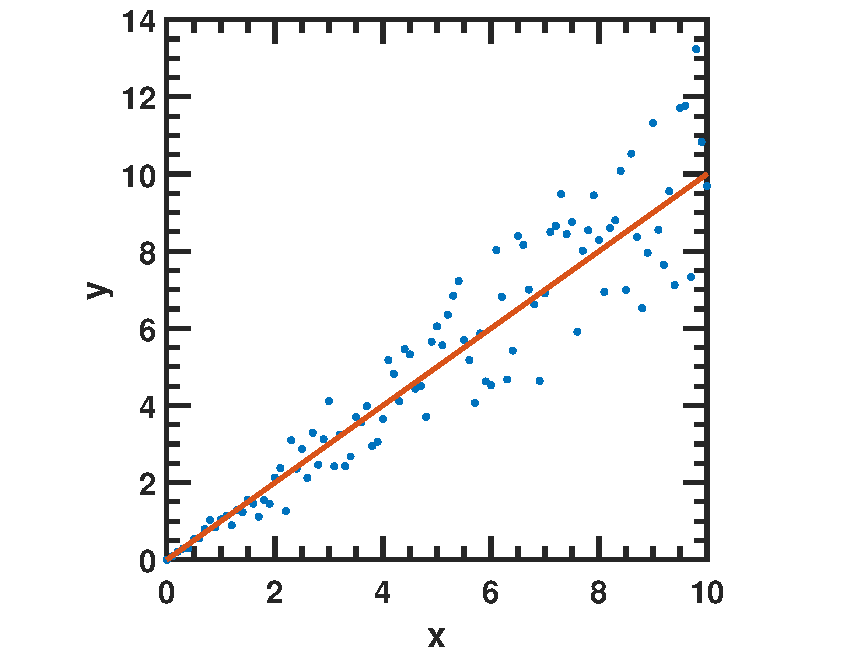
\includegraphics[width=0.6\linewidth]{../figures/statisticalModeling/estimationTheory/heteroscedasiticityDemo}
	\caption{Demo of heteroskedasticity in linear regression. The noises are larger at larger $x$ values.}
	\label{fig:heteroscedasiticitydemo}
\end{figure}



\begin{remark}[sources of heteroskedasticity and graphical features]
	
\end{remark}


\begin{remark}[consequences of heteroscedasticity]
OLS estimator is still unbiased. However, it is no longer efficient and t, F tests are no longer valid, as we discussed in \autoref{ch:regression-analysis:remark:propertiesOLSwithStructuralError}.
\end{remark}




\subsubsection{Test for heteroskedasticity}
\begin{remark}[intuition for designing heteroskedasticity test]\hfill
\begin{itemize}
	\item 	In the standard linear regression assumption, we have the homoskedasiticity assumption given by	
	$$Var[\epsilon|X] = E[\epsilon^2|X]= \sigma^2.$$
	\item To test the violation of this assumption, we want to test whether expected value of $u^2$ is related to one or more of the explanatory variables via certain function form (e.g., linear, quadratic, etc). 
	\item Therefore, we can ultimately test the relation by regressing $u^2$ on explanatory variables. 
\end{itemize}	
\end{remark}





\begin{method}[test for heteroskedasticity]\cite[280]{wooldridge2015introductory}
\begin{itemize}
	\item Estimate the model using OLS and obtain the residual estimates $\hat{\epsilon}$ and fitted value $\hat{y}$. 
	\item Run one of the following regression models:
	\begin{itemize}
		\item $\hat{\epsilon}^2 = \delta_0 + \delta_1x_1 + ... + \delta_k x_k + v.$
\item $\hat{\epsilon}^2 = \delta_0 + \delta_1x_1 + ... + \delta_k x_k + \delta_{k+1}x_1^2 + \delta_{k+2}x_1x_2 + ... +\delta_{k^2} x_k^2 + v.$
\item $\hat{\epsilon} = \delta_0 + \delta_1\hat{y} + \delta_2 \hat{y}^2 + v.$
	\end{itemize}
	\item Use $F$ or Lagrange multiplier test to see if $\delta_i, i=1,2,...$ are significantly different from zero. 
\end{itemize}	
\end{method}



\subsubsection{Heteroskedasticity robust estimator}

\begin{remark}[motivation and general remarks]\hfill
\begin{itemize}
	\item For a linear regression model with \textbf{known} structural error characterized by $Var[\epsilon] = \sigma^2 \Sigma$, we can use generalized least square method to estimate the coefficient and its standard error (\autoref{ch:statistical-models:th:GeneralizedLeastSquareSolution}). 
	\item If $\Omega$ is unknown, an 
	
	Robust standard errors is a technique to obtain unbiased standard errors of OLS coefficients under heteroscedasticity.
	\item If $\Omega$, another way is to use feasible GLS or feasible weighted least square. 
\end{itemize}	
\end{remark}



\begin{definition}[heteroscedasticity consistent standard error estimator, robust standard error estimator]
A typical heteroscedasticity consistent standard error estimator for $\beta$ is defined by	
	$$Var[\hat{\beta}] = (X^TX)^{-1}X^T\hat{\Sigma}X(X^TX)^{-1}$$
where $\hat{\Sigma}$ is given by
$$\hat{\Sigma} = \begin{bmatrix}
\hat{\epsilon}_1^2 &  &  & \\ 
& \hat{\epsilon}_2^2 &  & \\ 
&  & \ddots & \\ 
&  &  & \hat{\epsilon}_n^2
\end{bmatrix}, \hat{\epsilon}_i^2 = (y_i - \hat{\beta}x_i)^2.$$
Some variants will multiply $\hat{\Sigma}$ by $n/n-p$ as a degree-of-freedom correction.  
\end{definition}

\begin{remark}
For a linear regression model with structural error characterized by $Var[\epsilon] = \sigma^2 \Sigma$, the OLS estimator is given by (\autoref{ch:regression-analysis:remark:propertiesOLSwithStructuralError})	
	$$Var[\hat{\beta}] = \sigma^2 (X^TX)^{-1}X^T\Sigma X(X^TX)^{-1}.$$
\end{remark}



\subsubsection{Feasible weighted least square}

\begin{remark}[weighted least square as a special generalized least square]\index{weighted least square}
	Weighted least square is the special case that $\Sigma^{-1}=diag(w_1,...,w_p)$.
\end{remark}



\begin{algorithm}[H]
	\SetAlgoLined
	\KwIn{Data set consists of $X,Y$}
	Start with initial weight $w_i\geq 0,i=1,...,p$ and the error model, for example $var(\epsilon_i) = \gamma_0 + \gamma_1x_1$.\\
	Use generalized least square to estimate $\beta$.\\
	Use the residuals to estimate $\gamma$, by regressing $x$ on the residual $\hat{\epsilon}^2$.\\
	Re-compute the weights and go to step 2.\\
	\KwOut{The coefficients $\beta$}
	\caption{EM algorithm for least square with nonconstant variance}
\end{algorithm}


\begin{example}
Consider a simple regression problem for the following observations
\begin{center}
	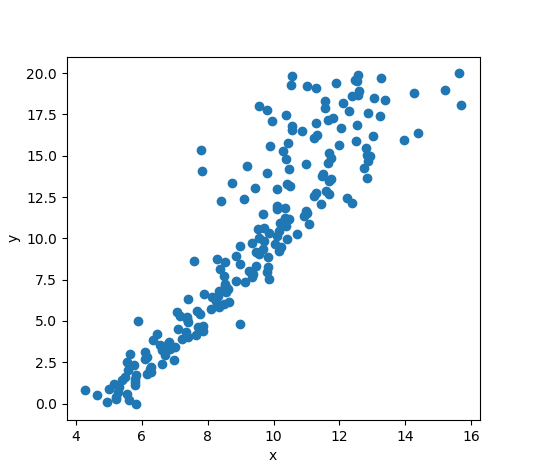
\includegraphics[width=0.5\linewidth]{../figures/statisticalModeling/regressionAnalysis/WLSDemo}
\end{center}
with is generated from $y = 5 + 0.5x + w(x) Z, Z\sim N(0, 0.25)$ and $w(x) = 1$ if $0 < x < 12$ else $w(x) = 3$. 

The estimated coefficients based on OLS ($\hat{\beta} = (X^TX)^{-1}X^TY$)and WLS  ($\hat{\beta} = (X^T\Sigma^{-1} X)^{-1}X^T\Sigma^{-1}Y$) are given in the following

\begin{Verbatim}[fontsize=\small]


OLS result
				coef    std err          t      P>|t|      
--------------------------------------------------------
const          5.1420      0.141     36.523      0.000  
x1             0.4847      0.012     39.802      0.000  
========================================================


WLS result
				coef    std err          t      P>|t|      
----------------------------------------------------------
const          5.0957      0.082     62.054      0.000    
x1             0.4951      0.010     47.732      0.000    
==========================================================

\end{Verbatim}
	

	
	
	
	
\end{example}



\subsection{Residual normality test}

\subsubsection{Jarque-Bera test}\index{Jarque-Bera test}

\begin{definition}[Jarque–Bera test]
Jarque–Bera test is a goodness-of-fit test of whether sample data have the skewness and kurtosis matching a normal distribution. The test statistic JB is defined as
	$$JB = \frac{n-k-1}{6}(S^2 + \frac{1}{4}(C-3)^2),$$
where $n$ is the number of observations, $S$ is the sample skewness, $C$ is the sample kurtosis, and $k$ is the number of regressors (excluding the constant regressor). Note that for a normal distribution, $S = 0$ and $C = 3$. 	
\end{definition}

\begin{remark}
If the data comes from a normal distribution, the JB statistic asymptotically has a $\chi^2(2)$ distribution, so the statistic can be used to test the hypothesis that the data are from a normal distribution.
\end{remark}


\subsubsection{D'Agostino's $K^2$ test}

\begin{definition}[D'Agostino's $K^2$ test]
D'Agostino's $K^2$ test is a goodness-of-fit test of whether the sample data's distribution deviate from normality. The statistic $K^2$ is defined by
$$K^2 = Z_1(g_1)^2 + Z_2(g_2)^2,$$
where $Z_1, Z_2$ are some transformation functions and $g_1, g_2$ are the sample skewness and sample kurtosis.	
\end{definition}

\begin{remark}
	If the data comes from a normal distribution, the $K^2$ statistic asymptotically has a $\chi^2(2)$ distribution, so the statistic can be used to test the hypothesis that the data are from a normal distribution.
\end{remark}



\subsection{Autocorrelation of errors and models}

\subsubsection{Motivation and general remarks}

\begin{remark}[source of autocorrelated error]
Suppose we have built a linear regression model to explain the GDP $Y$ using capital $K$, labor $L$, and technology $L$ over a period of time. The model is given by
$$\log(Y) = \beta_0 + \beta_1 \cdot K + \beta_2 \cdot L + \beta_3 \cdot L + \epsilon.$$

The unmodeled effects, such as policy effect, is adsorbed into the error term $\epsilon$. However, because policy in previous years usually can have impact on subsequent years, their effects, as included in $\epsilon$, can display autocorrelation effects.		
\end{remark}

\begin{remark}[consequences of autocorrelated error]
	OLS estimator is still unbiased. However, it is no longer efficient and t, F tests are no longer valid, as we discussed in \autoref{ch:regression-analysis:remark:propertiesOLSwithStructuralError}.
\end{remark}
\subsubsection{Test of autocorrelation of errors}



\begin{method}[linear regression coefficient test method for AR(1)]\cite[417]{wooldridge2015introductory}\hfill
\begin{itemize}
	\item Run the OLS regression and obtain the OLS residual $\hat{\epsilon}_i,i=1,2,...,n$.
	\item Run the regression
	$$\hat{\epsilon}_i = C + \hat{\rho}\hat{\epsilon}_{i-1},i=2,...,n.$$
	\item Use t test to test hypothesis $H_0: \rho = 0; H_1: \rho \neq 0$.
\end{itemize}	
\end{method}






\begin{method}[Durbin-Watson test]\index{Durbin-Watson test}
Let $\hat{a}$	
	$$d = \frac{\sum_{t=2}^T (e_t - e_{t-1})^2}{\sum_{t=1}^T e_t^2}$$
	where $e_t = y_t - \hat{y}_t$.
	The decision rule is given as
	\begin{itemize}
		\item 	If $d < d_{L,\alpha}$, there is statistical evidence that the error terms are positively autocorrelated.
		\item 	If $d > d_{U,\alpha}$, there is no evidence of autocorrelation.
		\item 	If $d_{L,\alpha} < d < d_{U,\alpha}$, the test is inconclusive.
	\end{itemize}
\end{method}

\begin{remark}[noise/error model]
	Durbin-Waston test assumes that the errors
	in the regression model are generated by AR(1) as, that is,
	$$e_{t} = \phi e_{t-1} + \eta,\eta\sim WN(0,\sigma^2),\abs{\phi}<1.$$
\end{remark}

\begin{remark}[interpretation]\hfill
	\begin{itemize}
		\item Durbin Watson test is a test that tests  autocorrelation in the residuals from a statistical regression analysis.
		\item The Durbin Watson statistic has the following approximation:
		\begin{align*}
		d &= \frac{\sum_{t=2}^T (e_t - e_{t-1})^2}{\sum_{t=1}^T e_t^2} \\
		  &= \frac{\sum_{t=2}^T e_t^2}{\sum_{t=1}^T e_t^2}+\frac{\sum_{t=2}^T e_t^2}{\sum_{t=1}^T e_t^2} - 2\frac{\sum_{t=2}^T e_te_{t-1}}{\sum_{t=1}^T e_t^2} \\
		  &\approx 1 + 1 - 2\frac{\sum_{t=2}^T e_te_{t-1}}{\sum_{t=1}^T e_t^2}\approx 2(1 - \phi).
		\end{align*}
		where $\phi$ is the AR(1) coefficient.
		\item The Durbin-Watson statistic is always between 0 and 4. A value of 2 means that there is no autocorrelation in the sample. Values approaching 0 indicate positive autocorrelation and values toward 4 indicate negative autocorrelation.
	\end{itemize}
\end{remark}

\begin{remark}[higher order model of errors]
	There are tests for higher order model of errors, such as Breusch-Pagan test.
\end{remark}


\subsubsection{Modeling autocorrelations}



\begin{definition}[linear regression model with AR(1) error]\cite[361]{hill2010principles}
The linear regression model for random variable $y_t$ depending on non-random observation $x$ and correlated error $e_t$ is given by 	
\begin{align*}
y_t &= \beta_0 + \beta_1 x_t + e_t \\
e_t & = \rho e_{t-1} + v_t
\end{align*}
where	
\begin{itemize}
	\item $-1< \rho < 1$
	\item $E[v_t] = 0, Var[v_t] = \sigma_v^2, Cov(v_s,v_t) = 0, \forall t\neq s$.
\end{itemize}
\end{definition}

\begin{remark}[View $y_t$ as a random variable and a random process]

\end{remark}


\begin{lemma}[equivalent form for auto-correlated AR(1) noise  model]\cite[361]{hill2010principles}\label{ch:regression-analysis:th:equivalentFormAR(1)NoiseModel}
The model 	
\begin{align*}
y_t &= \beta_0 + \beta_1 x_t + e_t \\
e_t & = \rho e_{t-1} + v_t
\end{align*}
has the following equivalent forms:
\begin{itemize}
	\item $$y_t = \beta_0 + \beta_1 x_t + \sum_{i=0}^\infty \rho^i v_{t-i};$$
	\item $$(1 - \rho B)y_t = \beta_0 + \beta_1(1 - \rho B) x_t  + v_t,$$
	where $B$ is the lag operator;
	\item $$y_t = \beta_0(1 - \rho) + \beta_1 x_t + \rho y_{t-1} - \rho \beta_1 x_{t-1} + v_t,$$
	or written by
	$$\tilde{y}_t = \beta_0(1 - \rho) + \beta_1 \tilde{x}_t  + v_t,$$
	where $\tilde{y}_t = y_t  - \rho y_{t-1}$ and $\tilde{x}_t = x_t - \rho x_{t-1}$. 
\end{itemize} 
\end{lemma}
\begin{proof}
	(1) Note that 
\begin{align*}
	(1 - \rho B) e_t= v_t \implies e_t  &=(1 - \rho B)^{-1} v_t \\
	& =  \sum_{i=0}^\infty \rho^i v_{t-i}
\end{align*}
(2)(3) Multiply both sides by $(1 - \rho B)$ will get the result.	
\end{proof}


\begin{remark}[alternative models]
We can also model the correlated $e_t$ using MA(q) and ARMA(p,q) model.	
\end{remark}


\subsubsection{Autoregressive transformation}

\begin{lemma}[autoregressive transformation to weighted least square]\cite[254]{theil1971principles}

If the error term satisfying 
$$\epsilon_i = \rho \epsilon_{i-1} + \xi_i, i = 2,3,...,n$$
where $n$ is the number of samples, $\abs{\rho}\leq 1$ is \textbf{known} and $E[\xi_i] = 0, E[\xi_i,\xi_j] = \sigma_0^2\delta_{ij}$. Then
\begin{itemize}
	\item $$E[\epsilon_i] = 0$$
	\item $$E[\epsilon_i\epsilon_j] = \sigma_0^2 \frac{\rho^{\abs{i-j}}}{1- \rho^2}.$$
\end{itemize}
Or equivalently, the $Cov[\epsilon,\epsilon] = \sigma_0^2 V$, where
$$V = \begin{pmatrix}
1 & \rho & \rho^2 & \cdots & \rho^{n-1}\\ 
\rho & 1 & \rho & \cdots & \rho^{n-2} \\ 
\rho^2 & \rho & 1 &  & \rho^{n-3}\\ 
\vdots &  &  & \ddots & \\ 
\rho^{n-1} & \rho^{n-2} & \rho^{n-3} & \cdots & 1 
\end{pmatrix}$$
	
\end{lemma}
\begin{proof}
Use the basic statistical properties in \autoref{ch:time-series-analysis:th:AR(1)processBasicProperties}.
\end{proof}



\begin{remark}[property of $V$ matrix]\hfill
Here we list some properties of $V$, which will be useful when we do weighted least square.	
\begin{itemize}
	\item $$V^{-1} = \frac{1}{1-\rho^2}\begin{pmatrix}
	1 & -\rho & 0 & \cdots & 0 & 0\\ 
	-\rho & 1+\rho^2 & -\rho & \cdots & 0 & 0\\ 
	0 & -\rho & 1+\rho^2 &  & 0 & 0\\ 
	\vdots & \vdots & \vdots &  & \vdots & \vdots\\ 
	0 & 0 & 0 & \cdots & 1+\rho^2 & -\rho\\ 
	0 & 0 & 0 & \cdots & -\rho & 1
	\end{pmatrix}$$
	\item $$V^{-1} = P^TP, P =\frac{1}{\sqrt{1-\rho^2}} \begin{pmatrix}
	\sqrt{1-\rho^2} & 0 & 0 & \cdots & 0 & 0\\ 
	-\rho & 1 & 0 & \cdots & 0 & 0\\ 
	0 & -\rho & 1 & \cdots & 0 & 0\\ 
	\vdots &  &  &  &  & \\ 
	0 & 0 & 0 & \cdots & 1 & 0 \\ 
	0 & 0 & 0 & \cdots & -\rho & 1
	\end{pmatrix}$$
	
\end{itemize}	
	
	
\end{remark}



\begin{remark}[when $\rho$ is unknown]\cite[254]{theil1971principles}
If we do not know $\rho$, we can use least square to estimate  the correlation]\autoref{ch:time-series-analysis:th:leastSquareEstimationOfCorrelationAR(1)}.
		The correlation parameter $\rho$ as a solution to	
		$$\min_{\rho} \sum_{i=2}^N (e_i - \rho e_{i-1})^2$$
		is given by
		$$\hat{\rho} = \frac{\sum_{t=1}^{N-1} e_t e_{t+1}}{\sum_{t=1}^{N-1} e_t^2},$$
		where $e_i$ is the residue from the standard least square solution.	
\end{remark}

\subsubsection{Feasible GLS for unknown correlation}

\begin{method}[feasible GLS for AR(1) ]\cite[425]{wooldridge2015introductory}
\begin{itemize}
	\item Perform OLS estimator and obtain the residual $\hat{\epsilon}_i, i=1,2,...,n$.
	\item Regress $\hat{\epsilon}_i$ on $\hat{\epsilon}_{i-1}$ to obtain $\hat{\rho}$
	\item Construct the estimated $\hat{\Sigma}$, and use GLS estimator
	
	or apply OLS estimation to the equivalent form in \autoref{ch:regression-analysis:th:equivalentFormAR(1)NoiseModel}.
\end{itemize}
\end{method}

\subsection{Rank deficiency and penalized linear regression}

If the number of predicators is exceeding the number of observations, the ordinary linear regression will break down since the matrix $X$ does not have full column rank and $X^TX$ has rank deficiency. In such case, we can use penalized linear regression discussed in \autoref{ch:statistical-learning-linear-models:sec:PenalizedLinearRegression}.

\subsection{Outliers and Robust linear regression}

\subsubsection{Outliers and influential points}

\begin{definition}[outlier, high leverage point, influential point]\hfill
\begin{itemize}
	\item An \textbf{outlier} is a data point whose response y does not follow the general trend of the rest of the data.
	\item A data point has \textbf{high leverage} if it has "extreme" predictor x values.
	\item A data point is \textbf{influential} if it affects the predicted responses significantly via the estimated slope coefficients Outliers and high leverage data points have the potential to be influential, but not necessarily so.
\end{itemize}	
\end{definition}


\begin{definition}[leverage]
Let $H$ be the orthogonal projector matrix in the multiple linear regression. $H_{ii}$ is called the \textbf{leverage point} because $H_ii$ quantifies the influence that the observed response $y_i$ has on the predicted response $\hat{y}_i$ since
$$\hat{y}_i = H_{i1}y_1 + \cdots + H_{ii}y_i + \cdots + H_{in}y_n.$$	
\end{definition}

\begin{figure}[H]
	\centering
	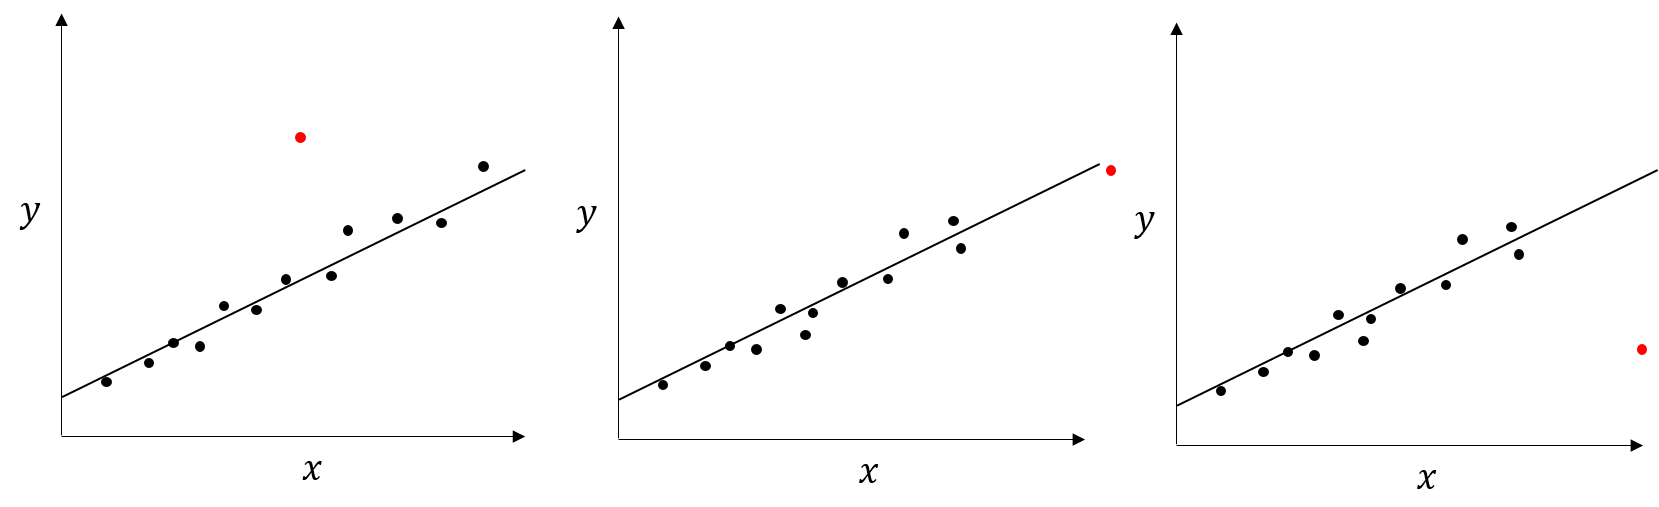
\includegraphics[width=1\linewidth]{../figures/statisticalModeling/regressionAnalysis/influencePointsLinearRegression}
	\caption{Illustration of an outlier, a high-leverage point, and a influential point. Left subfigure shows a red-colored outlier, which does not have high leverage and large influence on the regression result. Middle subfigure shows a red-colored high-leverage point, which is not an outlier or influential point due to its weak influence on the regression result. Right subfigure shows an influential point that is both an outlier and a high-leverage point.}
	\label{fig:influencepointslinearregression}
\end{figure}


\begin{note}[interpretation and usage of leverage to identify influential points]\hfill
\begin{itemize}
	\item That is, if $H_{ii}$ is small, then the observed response $y_i$ plays only a small role in the value of the predicted response $\hat{y}_i$; On the other hand, if $H_{ii}$ is large, then the observed response $y_i$ plays a large role in the value of the predicted response $\hat{y}_i$.
	\item $H_{ii}$ is between 0 and 1, inclusively; and $\sum_i H_{ii} = p$.(\autoref{ch:linearalgebra:th:spectralpropertyorthogonalprojector})
	\item If $$H_{ii} > 3\frac{\sum_i H_{ii}}{n} = 3\frac{p}{n},$$
	that is, $H_{ii}$ is more than 3 times larger than the mean leverage value, we identify the pair $(x_i,y_i)$ as the influential points. 
\end{itemize}	
\end{note}






\subsubsection{Robust regression}



\begin{lemma}[robust estimator]
The robust estimator for the parameter $\beta$ is obtained by solving the following optimization problem	
$$\min_{\beta \in \R^p} \sum_{i=1}^{n} \rho(e_i) = \min_{\beta} \sum_{i=1}^{n} \rho(y_i - x_i^T\beta),$$
where the function $\rho$ is related the likelihood function for an appropriate choice of the error distribution.

An alternative scale-invariant optimization formulation is given by
$$\min_{\beta \in \R^p} \sum_{i=1}^{n} \rho(\frac{e_i}{s}) = \min_{\beta} \sum_{i=1}^{n} \rho(\frac{y_i - x_i^T\beta}{s}),$$
where $s$ is a robust estimate of scale. A popular choice for $s$ is the median absolute deviation(\autoref{ch:theory-of-statistics:def:medianabsoluteDeviation})
$$s = median[e_i - median[e_i]]/0.6745.$$	
\end{lemma}


\begin{example}[example functions]\hfill
	\begin{itemize}
		\item (least square) $$\rho(z) = \frac{1}{2}z^2, \psi(z) = z.$$
		\item (Huber's t function)
		$$\rho(z) = 
		\begin{cases*}
		\frac{1}{2}z^2, \abs{z} \leq t \\
		0, otherwise
		\end{cases*}.$$
		\item (Cauchy)
		$$\rho(z) = \frac{1}{1+z^2}.$$ 
	\end{itemize}
\end{example}



\begin{lemma}[iteratively reweighted least square approach for parameter estimation]\cite[373]{montgomery2012introduction}
Consider a robust estimator by solving the following problem given by
$$\min_{\beta \in \R^p} \sum_{i=1}^{n} \rho(\frac{e_i}{s}) = \min_{\beta} \sum_{i=1}^{n} \rho(\frac{y_i - x_i^T\beta}{s}).$$
\begin{itemize}
	\item The first order necessary condition for the minimum is given by
	$$\sum_{i=1}^{n} x_{ij}\psi((y_i-x_i^T\beta)/s),$$
where $\psi = \rho'$ and $x_{ij}$ is the i observation on the j regressor and $x_{i0}=1$.	
\item (iterative reweighted algorithm) The iterative reweighted algorithm is formulated using the old estimated $\hat{\beta}_0$ and solve for the new iterate $\beta$ via
	$$\sum_{i=1}^{n} x_{ij}w_{i0}\cdot (y_i-x_i^T\beta) = 0, j=0,1,...,k; (*)$$
where 
$$w_{i0} = \begin{cases*}
\frac{\psi[(y_i-x_i^T\hat{\beta}_0)/s]}{(y_i-x_i^T\hat{\beta}_0)/s}, if~y_i\neq x_i^T\hat{\beta}_0 \\
1
\end{cases*}$$	

In matrix form, $(*)$ is given by
$$X^TW_0X\beta = X^TW_0y,$$
where $W_0$ is an $n\times n$ diagonal matrix of weights with diagonal elements $w_{10},w_{20},...,w_{n0}$. 
And the new minimizer iterate is given by
$$\hat{\beta}_1 = (X^TW_0X)^{-1}X^TW_0y.$$
\end{itemize}
\end{lemma}


\subsubsection{Least absolute deviation (LAD) regression}

\begin{definition}[multiple linear regression with least absolute deviations]\label{ch:statistical-models:th:multipleLinearRegressionLeastAbsoluteDeviation}	The multiple linear regression model \textbf{assumes} that a random variable $Y$ has a linear dependency on a non-random vector $X = (X_1,X_2,...,X_{p-1}) \in \R^{p-1}$ given as
	$$Y = \beta_0 + \beta_1 X_1 +\beta_2 X_2 + ... +\beta_{p-1} X_{p-1} + \epsilon.$$
	Given the observed sample pairs $(x_1,y_1),(x_2,y_2),..., (x_n,y_n), x\in \R^{p-1}, y\in \R$ as $y_i = \beta_0 + \beta_1 x_{i1} + \beta_2 x_{i2} + ... + \epsilon_i$ and we \textbf{further make the following assumptions on $\epsilon$} as
	\begin{itemize}
		\item $E[\epsilon_i] = 0,\forall i$
		\item $cov(\epsilon_i,\epsilon_j) = \sigma^2\delta_{ij}$ and $\sigma^2$ is unknown.
	\end{itemize} 	
	
	The least absolute deviation estimation of the coefficient $\beta_0,\beta_1,...,\beta_p$ is from the optimization
	$$\min_{\beta_0,\beta_1,...,\beta_p} \sum_{i=1}^{n} \abs{y_i - \beta_0 - \beta_1 x_{i1} - \beta_2 x_{i2} - \cdots -\beta_p x_{ip}}.$$
\end{definition}

\begin{remark}[motivation and issues with least absolute deviation optimization]\hfill
\begin{itemize}
	\item LAD regression is robust to outliers, whereas least square regression is not.
	\item LAD regression might give multiple solution due to its linear programming nature.
\end{itemize}	
\end{remark}


\begin{lemma}[solution via linear programming]
The optimization problem given by
$$\min_{a_0,a_1,...,a_k} \sum_{i=1}^{n} \abs{y_i - a_0 - a_1 x_{i1} - a_2 x_{i2} - \cdots -a_k x_{ik}},$$
can be transformed to the following linear programming problem
\begin{align*}
&\min_{a_0,a_1,...,a_k, u_1,...,u_n} \sum_{i=1}^{n} u_i ,\\
s.t. & u_i \geq y_i - a_0 -a_1x_{i1} -a_2x_{i2} - \cdots -a_kx_{ik}, i=1,...,n. \\
& u_i \geq -(y_i - a_0 -a_1x_{i1} -a_2x_{i2} - \cdots -a_kx_{ik}), i=1,...,n. 
\end{align*}
\end{lemma}
\begin{proof}
Todo
\end{proof}


\subsection{Quantile regression}\index{quantile regression}

\begin{lemma}[sample quantile as the solution to an optimization problem]\cite[87]{cameron2005microeconometrics} 
The sample $q$th quantile, denoted by $\hat{\mu}_q$, is also the solution to the following optimization problem
$$\min_{\beta \in \R} \sum_{i:y_i\geq \beta}^{N} q\abs{y_i-\beta} + \sum_{i:y_i < \beta}^{max}(1-q)\abs{y_i-\beta};$$
or equivalently
$$\min_{\beta \in \R} \sum_{i=1}^{N} (q-\bm{1}_{y_i<\beta})\abs{y_i-\beta}.$$

In particular, if $q=0.5$,i.e., median, then the median is the minimum of the following optimization
$$\min_{\beta \in \R} \sum_{i:y_i\geq \beta}^{N} \abs{y_i-\beta}.$$
\end{lemma}


\begin{remark}[the intuition for median]\hfill
\begin{itemize}
	\item 
	Suppose in a sample of 99 observations that the 50th smallest observations,i.e. the median, equals 10 and the 51st smallest observation equals 12. 
	\item 
	If we let $\beta = 12$, then the first 50 ordered observations will increase by 2 and the remaining 49 observations will decrease by 2, leading to an overall net increase of $$50\times 2 - 49\times 2 = 2.$$
	\item Similarly, the 49th smallest observation can be shown to be a worse choice compared with the 50th observation.
\end{itemize}	 	
\end{remark}

\begin{definition}\cite[87]{cameron2005microeconometrics} 
	The multiple linear regression model \textbf{assumes} that a random variable $Y$ has a linear dependency on a non-random vector $X = (X_1,X_2,...,X_{p-1}) \in \R^{p-1}$ given as
	$$Y = \beta_0 + \beta_1 X_1 +\beta_2 X_2 + ... +\beta_{p-1} X_{p-1} + \epsilon.$$
	Given the observed sample pairs $(x_1,y_1),(x_2,y_2),..., (x_n,y_n), x\in \R^{p-1}, y\in \R$ as $y_i = \beta_0 + \beta_1 x_{i1} + \beta_2 x_{i2} + ... + \epsilon_i$ and we \textbf{further make the following assumptions on $\epsilon$} as
	\begin{itemize}
		\item $E[\epsilon_i] = 0,\forall i$
		\item $cov(\epsilon_i,\epsilon_j) = \sigma^2\delta_{ij}$ and $\sigma^2$ is unknown.
	\end{itemize} 	
	
The $q$th \textbf{quantile multiple linear regression estimator $\hat{\beta}_q$} minimizes the following the optimization problem
$$\min_{\beta \in \R^q} \sum_{i:y_i\geq x_i^T\beta}^{N} q\abs{y_i-x_i^T\beta} + \sum_{i:y_i < \beta}^{max}(1-q)\abs{y_i-x_i^T\beta};$$
or equivalently
$$\min_{\beta \in \R^n} \sum_{i=1}^{N} (q-\bm{1}_{y_i<\beta^Tx_i})\abs{y_i-\beta^Tx_i}.$$

\end{definition}

\begin{remark}[special case of least absolute deviation estimator]
When $q = 0.5$, we will get the median, the regression problem becomes the least absolute deviation regression(\autoref{ch:statistical-models:th:multipleLinearRegressionLeastAbsoluteDeviation}). 
\end{remark}


\subsection{Regressor correlation with error}

\subsubsection{Problems with ordinary least square estimator}

\begin{lemma}[ordinary least square estimator is biased]
In the multiple linear regression, the ordinary least square estimator given by
$$\hat{\beta} = (X^TX)^{-1}X^TY,$$
will be biased if $Cov(X,\epsilon) > 0.$
That is
$$E[\hat{\beta}] \neq \beta.$$	
\end{lemma}
\begin{proof}
$$E[\hat{\beta}] = (X^TX)^{-1}X^T(X\beta+\epsilon) = \beta + (X^TX)^{-1}X^T\epsilon\neq \beta.$$	
\end{proof}

\subsubsection{Reasons leading to correlation}

\begin{remark}[correlation due to omitted variables]
\cite[407]{hill2008principles}
Suppose the true model between $Y$ and $X_1,X_2,...,X_n$ is given by
$$Y = \beta_1X_1+\beta_2X_2+...+\beta_nX_n + \epsilon,$$
where $\epsilon$ is independent of $Y$ and $X$s, and $X_1,X_2,...,X_n$ be correlated. If we propose a model of 
$$Y = \alpha_1X_1+\alpha_2X_2+...+\alpha_{n-1}X_{n-1} + \eta,$$
then the $\eta$ will be correlated with $X_1,X_2,...,X_n$.	
\end{remark}


\begin{remark}[correlation due to measurement error]\cite[406]{hill2008principles}
Suppose our true model is given by
$$Y = \beta_1 + \beta_2 X^* + \epsilon,$$
where $\epsilon$ is independent of $X$. Now suppose
our model due to measurement error is given by
$$Y = \beta_1 + \beta_2 X + \eta,$$
where $X = X^* + u$, $u$ is the measurement error independent of $X$, and $\eta = \epsilon - \beta_2 u$.

Then $$Cov(X,\eta) = Cov(X^*+u,\epsilon-\beta_2 u) = -\beta Var[u].$$	
\end{remark}



\subsubsection{Instrument variable estimator}

\begin{lemma}
$$\hat{\beta} = (Z^TX)^{-1}Z^TY$$
is unbiased.

$$Var[\hat{\beta}] = (Z^TX)^{-1}Z^T\Omega Z(Z^TX)^{-1}.$$
\end{lemma}
\begin{align*}
\hat{\beta} &= (Z^TX)^{-1}Z^TY \\
&=(Z^TX)^{-1}Z^T(X\beta + \epsilon) \\
&=(Z^TX)^{-1}Z^TX\beta + (Z^TX)^{-1}Z^T\epsilon \\
&=\beta + 0\\
&=\beta
\end{align*}



\begin{lemma}
The two-stage least squares estimator can be compactly written as
$$\hat{\beta} = (X^TP_ZX)^{-1}(X^TP_ZY),$$
where $$P_Z = Z(Z^TZ)^{-1}Z^T$$
is the orthogonal projectors such that $P_Z^T=P_Z, P_Z^2 = P_Z.$	
\end{lemma}





\section{Linear regression case studies}

\subsection{Summary of OLS in different scenarios}
\href{https://www.asc.ohio-state.edu/de-jong.8/note5.pdf}{link}


\begin{description}
	\item[Case 1] OLS with deterministic regressors and iid Gaussian errors.
	\item[Case 2] OLS with stochastic regressors and iid Gaussian errors.
	\item[Case 3] OLS with stochastic regressors and iid Non-Gaussian errors.
	\item[Case 4] OLS with deterministic regressors and non-iid errors.
\end{description}




\subsection{Standard linear regression}



\begin{verbatim}
OLS Regression Results                            
==============================================================================
Dep. Variable:                      y   R-squared:                       0.878
Model:                            OLS   Adj. R-squared:                  0.877
Method:                 Least Squares   F-statistic:                     707.4
Date:                Tue, 30 Oct 2018   Prob (F-statistic):           1.29e-46
Time:                        23:08:39   Log-Likelihood:                 77.109
No. Observations:                 100   AIC:                            -150.2
Df Residuals:                      98   BIC:                            -145.0
Df Model:                           1                                         
Covariance Type:            nonrobust                                         
==============================================================================
                coef      std err       t        P>|t|      [0.025      0.975]
------------------------------------------------------------------------------
const          1.9841      0.022     88.410      0.000       1.940       2.029
x1             1.0312      0.039     26.596      0.000       0.954       1.108
==============================================================================
Omnibus:                        0.886   Durbin-Watson:                   2.028
Prob(Omnibus):                  0.642   Jarque-Bera (JB):                0.914
Skew:                           0.080   Prob(JB):                        0.633
Kurtosis:                       2.560   Cond. No.                         4.35
==============================================================================
\end{verbatim}

basic information about the model fit:
\begin{description}
	\item[Dep. Variable] Which variable is the response in the model
	\item[Model]	What model you are using in the fit
	\item[Method]	How the parameters of the model were calculated
	\item[No. Observations]	The number of observations (examples)
	\item[DF Residuals]	Degrees of freedom of the residuals. Number of observations - number of parameters
	\item[DF Model]	Number of parameters in the model (not including the constant term if present)
\end{description}	

 the goodness of fit
\begin{description}
	\item[R-squared] The coefficient of determination. A statistical measure of how well the regression line approximates the real data points
	\item[Adj. R-squared]	The above value adjusted based on the number of observations and the degrees-of-freedom of the residuals
	\item[F-statistic]	A measure how significant the fit is. The mean squared error of the model divided by the mean squared error of the residuals
	\item[Prob (F-statistic)]	The probability that you would get the above statistic, given the null hypothesis that they are unrelated
	\item[Log-likelihood]	The log of the likelihood function.
	\item[AIC]	The Akaike Information Criterion. Adjusts the log-likelihood based on the number of observations and the complexity of the model.
	\item[BIC]	The Bayesian Information Criterion. Similar to the AIC, but has a higher penalty for models with more parameters.
\end{description}	

each of the coefficients
\begin{description}
	\item[coef]	The estimated value of the coefficient
	\item[std err]	The basic standard error of the estimate of the coefficient. More sophisticated errors are also available.
	\item[t]	The t-statistic value. This is a measure of how statistically significant the coefficient is.
	\item[P > |t|]	P-value that the null-hypothesis that the coefficient = 0 is true. If it is less than the confidence level, often 0.05, it indicates that there is a statistically significant relationship between the term and the response.
	\item[95.0\% Conf. Interval]	
	The lower and upper values of the 95\% confidence interval
\end{description}	
	
	
	Finally, there are several statistical tests to assess the distribution of the residuals
	
\begin{description}
	\item[Skewness]	A measure of the symmetry of the data about the mean. Normally-distributed errors should be symmetrically distributed about the mean (equal amounts above and below the line).
	\item[Kurtosis]	A measure of the shape of the distribution. Compares the amount of data close to the mean with those far away from the mean (in the tails).
	\item[Omnibus]	D'Angostino's test. It provides a combined statistical test for the presence of skewness and kurtosis.
	\item[Prob(Omnibus)]	The above statistic turned into a probability
	\item[Jarque-Bera]	A different test of the skewness and kurtosis
	\item[Prob (JB)]	The above statistic turned into a probability
	\item[Durbin-Watson]	A test for the presence of autocorrelation (that the errors are not independent.) Often important in time-series analysis
	\item[Cond. No]	A test for multicollinearity (if in a fit with multiple parameters, the parameters are related with each other).
\end{description}


\section{Linear regression application examples}


\subsection{Categories of analysis}
\subsubsection{Time series data}

\begin{definition}[time series data]\index{time series data}
Time series data has the following characteristics:
\begin{itemize}
	\item Observations of features (weight, height, revenue, population, GDP) of a single entity (person, firm, country) are collected at multiple time periods.
	\item Order of the data is important and observations are typically not independent over time.
\end{itemize}		
\end{definition}


\begin{example}
Examples of time series data include:
\begin{itemize}
	\item GDP data of China from 1978 to 2008.
	\item Price levels (CPI) of the US from 1900 to 2016.
	\item Daily value of SP500  index from 1990 to 2018.  
\end{itemize}
\end{example}


\subsubsection{Cross-section data}


\begin{definition}[Cross-sectional data]
	Panel data has the following characteristics:
	\begin{itemize}
		\item Observations of features of multiple entities (individuals,firms, countries) at the same point of time (or observed at different point of time but the time difference is not important).
		\item No time dimension, and order of the data does not matter.
	\end{itemize}	
\end{definition}

\begin{example}
	Examples of cross-sectional data include:
	\begin{itemize}
		\item The weights and heights data from a random sample of 1000 people which is used to analyze the obesity level in a population. 
	\end{itemize}
\end{example}



\subsubsection{Panel data analysis}

\begin{definition}[panel data]
Panel data has the following characteristics:
\begin{itemize}
	\item Observations of features of multiple entities (individuals,firms, countries) at multiple points in time.
	\item Can be viewed as the combination of time series data and cross-sectional data.
\end{itemize}	
\end{definition}

\begin{example}
	Examples of panel data include:
	\begin{itemize}
		\item The daily stock price data of 500 preselected NYSE companies from 1990 to 2016.
		\item Price levels (CPI) of G8 countries from 1900 to 2016.
	\end{itemize}
\end{example}


\subsection{Cross-section analysis}



\subsection{Panel data analysis}



\section{Generalized linear model}
\subsubsection{Poisson regression}

\begin{definition}[Poisson regression]
In \textbf{Poisson regression}, the dependent variable $Y$ is an observed count that follows the Poisson distribution.
$$Pr(Y=y|\lambda) = \frac{\exp(-\lambda)\lambda^y}{y!},$$
for $y=0,1,2,...$
 The rate $\lambda$ is determined by a set $p-1$ predictors $X_1,X_2,...,X_{p-1}$. The expression relating these quantities is
 $$\lambda = \exp(X^T\beta),$$
where $X=(1,X_1,X_2,...,X_{p-1}).$ 	
\end{definition}


\begin{lemma}[likelihood function]
Consider a set of random sample given by $(X_1,y_1),(X_2,y_2),...,(X_n,y_n)$.
the likelihood function is given by
$$L(\beta;y,X) = \prod_i^n \frac{\exp(-\exp(X_i^T\beta))\exp(X_i^T\beta)^y_i}{y_i!}.$$

The log-likelihood function is given by
$$l(\beta;y,X) = \sum_{i=1}^n y_iX_i^T\beta - \sum_{i=1}^n \exp(X_i\beta) - \sum_{i=1}^{n}\log(y_i!).$$	
\end{lemma}



\begin{lemma}[goodness-of-fit chi-square test]
Consider a set of random sample given by $(X_1,y_1),(X_2,y_2),...,(X_n,y_n)$.
Let $\hat{\beta}$ be the estimated coefficient.
The \textbf{Person statistic} defined by
$$X^2 = \sum_{i=1}^{n}=\frac{y_i - \exp(X_i^T\hat{\beta})^2}{\exp(X_i\hat{\beta})},$$
is approximately chi-square distributed with $n-p$ degrees of freedom.	
\end{lemma}
\begin{proof}
Use Pearson's theorem in \autoref{ch:theory-of-statistics:th:PearsonTheorem}. To do: show that how $n-p$ arises?
\end{proof}



\section{Generalized moment methods}
\begin{method}[generalized moment method (GMM) estimation]
Consider the following setup:
\begin{itemize}
	\item Let $\beta$ denote a $p\times 1$ parameter vector, $x_i, i=1,2,...,n$ data observations.
	\item Let $g_i(\beta) \triangleq g_i(\{x_i\}, \beta), i=1,2...,m $ be $m$ functions of the data and parameters.
\end{itemize}	

Then the GMM estimator $\hat{\beta}$ for the true paramater $\beta_0$ is such that the $m$ moment conditions
$$E[g_i(\beta_0)] = 0, i=1,2,...,m.$$
are satisfied.

More formally, the GMM estimator $\hat{beta}$ is formulated as the minimizer of
$$\hat{\beta} = \arg\min_{\beta} \hat{g}(\beta)^T$$	
where $A$ denotes an $m\times m$ positive semi-definite matrix,
$$\hat{g}(\beta) = \frac{1}{n}$$	
\end{method}


\begin{example}
Consider the linear regression model
$$Y = X^T\beta_0 + u,$$
where $X = (X_1,...,X_p)^T$ is a random vector of $p$ regressors, $\beta_0$ is the unknown linear regression coefficient vector, and $u$ is the noise term. 
Consider the $p$ population moment condition 
$$E[X_i(Y - X^T\beta_0)] = 0, i=1,2,...,p,$$
which gives the $p$ sample moment condition
$$\frac{1}{n}\sum_{j=1}^n x_i^{(j)} \hat{u}_i = \frac{1}{n}\sum_{j=1}^n x_i^{(j)} (y_i - [x^{(j)}]^T\hat{\beta}) = 0, i=1,2,...,p.$$
\end{example}



\section{Multivariate multiple linear regression (MMLR)}


\subsection{Canonical MMLR}
\begin{definition}
The multivariate multiple linear regression model has the form
$$y_{ik} = \beta_{0k} + \sum_{j=1}^p \beta_{jk}x_{ij} + \epsilon_{ik},$$
for $i\in \{1,...,n\}$ and $k\in \{1,...,m\}$ where
\begin{itemize}
	\item $y_{ik}\in \R$ is the $k$th real-valued response for the $i$th observation.
	\item $\beta_{0k}\in \R$ is the regression intercept for $k$th response
	\item $\beta_{jk}\in \R$ is the $j$th predictor's regression slope for $k$th response
	\item $x_{ij}\in \R$ is the $j$th predictor for the $i$th observation
	\item random vector $(\epsilon_{i1},...,\epsilon_{im})\sim MN(0,\Sigma)$ 
\end{itemize}	

It can be written in the following matrix form
$$Y = XB + E,$$
where 
\begin{itemize}
	\item $Y\in \R^{n\times m}$ is the $n\times m$ response matrix. 
	\item $X = [\bm{1}, x_1,...,x_p] \in \R^{n\times (p+1)}$ is the $n\times (p+1)$ design matrix.
	\item $B$ is $(p+1)\times m$ matrix of coefficients.
	\item $E$ is the error matrix consisting of $n\times m$ random variables. 
\end{itemize}

In the expanded view, we have
$$\begin{pmatrix}
y_{11} & \cdots & y_{1m}\\ 
y_{21} & \cdots & y_{2m}\\
y_{31} & \cdots & y_{3m}\\
\vdots & \ddots & \vdots\\ 
y_{n1} & \cdots & y_{nm}
\end{pmatrix} = \begin{pmatrix}
1 & x_{11} & x_{12} & \cdots & x_{1p}\\ 
1 & x_{21} & x_{22} & \cdots & x_{2p}\\
1 & x_{31} & x_{32} & \cdots & x_{3p}\\
\vdots & \ddots & \vdots\\ 
1 & x_{n1} & x_{n2} & \cdots & x_{np}\\
\end{pmatrix}\begin{pmatrix}
	\beta_{01} & \cdots & \beta_{0m}\\ 
	\beta_{21} & \cdots & \beta_{1m}\\
	\beta_{31} & \cdots & \beta_{2m}\\
	\vdots & \ddots & \vdots\\ 
	\beta_{p1} & \cdots & \beta_{pm}
\end{pmatrix} + \begin{pmatrix}
e_{11} & \cdots & e_{1m}\\ 
e_{21} & \cdots & e_{2m}\\
e_{31} & \cdots & e_{3m}\\
\vdots & \ddots & \vdots\\ 
e_{n1} & \cdots & e_{nm}
\end{pmatrix} $$
\end{definition}


\begin{remark}[interpret the name]\hfill
\begin{itemize}
	\item The model is multivariate because we have $m > 1$ response variables.
	\item The model is multiple because we have $p > 1$ predictors. 
\end{itemize}	
\end{remark}


\begin{assumption}[Fundamental assumptions of the MMLR]\hfill
\begin{itemize}
	\item Relationship between $X_j$ and $Y_k$ is linear (given other predictors)
	\item $x_{ij}$ and $y_{ik}$ are observed random variables
	\item $(\epsilon_{i1},...,\epsilon_{im})\sim MN(0, \Sigma)$ is an unobserved random vector. 
	\item $\beta$s are unknown constants. 
	\item $(y_{ik}|x_{i1},...,x_{ip})\sim N(\beta_{0k} + \sum_{j=1}^p \beta_{jk}x_{ij}, \sigma_{kk})$ for each $k\in \{1,...,m\}$. That is, homogeneity of variance for each response. 
\end{itemize}	
\end{assumption}


\subsubsection{Ordinary least square solution}


\begin{theorem}[OLS problems]

$$\min_{B\in \R^{(p+1)\times m}} \norm{Y - XB}^2_F = \min_{B\in \R^{(p+1)\times m}} \sum_{i=1}^n \sum_{k=1}^m (y_{ik} - \beta_{0k} - \sum_{j=1}^p \beta_{jk}x_{ij})^2,$$
where
\begin{itemize}
	\item The objective function can be written by
	$$OLS(B) = \norm{Y - XB}^2_F = Tr(Y^TY) - 2Tr(Y^TXB) + Tr(B^TX^TXB).$$
	\item The first order derivative respect to $B$ is given by
	$$\frac{\Pa OLS(B)}{\Pa B} = -2X^TY + 2X^TXB.$$
	\item The OLS solution is given by
	$$\hat{B} = (X^TX)^{-1}X^TY;$$
	The $k$ column in $\hat{B}$ is given by
	$$\hat{\beta}_k = (X^TX)^{-1}X^Ty_k.$$
\end{itemize}	
\end{theorem}
\begin{proof}
Note that
$$\norm{Y - XB}^2_F = Tr((Y - XB)^T(Y-XB))$$
\end{proof}



\begin{example}[R example]\hfill
\begin{verbatim}
> head(mtcars)
mpg cyl disp  hp drat    wt  qsec vs am gear carb
Mazda RX4         21.0   6  160 110 3.90 2.620 16.46  0  1    4    4
Mazda RX4 Wag     21.0   6  160 110 3.90 2.875 17.02  0  1    4    4
Datsun 710        22.8   4  108  93 3.85 2.320 18.61  1  1    4    1
Hornet 4 Drive    21.4   6  258 110 3.08 3.215 19.44  1  0    3    1
Hornet Sportabout 18.7   8  360 175 3.15 3.440 17.02  0  0    3    2
Valiant           18.1   6  225 105 2.76 3.460 20.22  1  0    3    1
> mtcars$cyl <- as.factor(mtcars$cyl)
> Y <- as.matrix(mtcars[,c("mpg","disp","hp", "wt")])
> coef(lm(Y ~ cyl + am + carb, data = mtcars))
mpg      disp         hp         wt
(Intercept) 25.320303 134.32487 46.5201421  2.7612069
cyl6        -3.549419  61.84324  0.9116288  0.1957229
cyl8        -6.904637 218.99063 87.5910956  0.7723077
am           4.226774 -43.80256  4.4472569 -1.0254749
carb        -1.119855   1.72629 21.2764930  0.1749132
\end{verbatim}	
\end{example}

\begin{remark}
For discussion in hypothesis testing, see \href{http://users.stat.umn.edu/~helwig/notes/mvlr-Notes.pdf}{link} and \cite{velu1998multivariate}. 
\end{remark}

\subsection{Seemingly unrelated regression model}






\subsection{Reduced rank regression}

\begin{definition}[reduced rank regression]
Consider a multivariate multiple linear regression. Let $X$ and $Y$ be centered predictor $(n\times p)$and response $(n\times q)$ data matrices. Then ordinary least squares (OLS) solution for reduced-rank regression can be formulated as minimizing the following cost function:
$$\min_{B\in \R^{(p)\times m}, rank(B)\leq r} \norm{Y - XB}^2_F = \min_{B\in \R^{(p+1)\times m}} \sum_{i=1}^n \sum_{k=1}^m (y_{ik} - \beta_{0k} - \sum_{j=1}^p \beta_{jk}x_{ij})^2. $$	
\end{definition}


\begin{theorem}[OLS solution to reduced rank regression]
Consider a multivariate multiple linear regression with $X\in \R^{n\times p}$ and $Y\in \R^{n\times m}$. Assume $(X^TX)$ is non-singular. 	
	Then the minimizer for the optimization
	$$\min_{B\in \R^{p\times m}, rank(B)\leq r} \norm{Y - XB}_F^2 = Tr[(Y - XB)^T(Y-XB)]$$
	is given by
	$$\hat{B} = (X^TX)^{-1}X^TYV_rV_r^T,$$
	where $V_r \in \R^{m\times r}$ whose columns are the top $r$ eigenvectors of $Y^TX(X^TX)^{-1}X^TY$
\end{theorem}
\begin{proof}
\begin{align*}
 &\norm{Y - XB}^2 \\
=& Tr[(Y  -XB)^T(Y - XB)] \\
=& Tr[(Y^TY - Y^TXB - B^TX^TY + B^TX^TXB)] \\
=& Tr[Y^TY - Y^TX(X^TX)^{-1}X^TY] + Tr[((X^TX)^{-1/2}X^TY - \\ &(X^TX)^{1/2}B)^T((X^TX)^{-1/2}X^TY - (X^TX)^{1/2}B)] \\
=& Tr[Y^TY - Y^TX(X^TX)^{-1}X^TY] + \norm{(X^TX)^{-1/2}X^TY - (X^TX)^{1/2}B}_F^2 
\end{align*}
Based on low rank approximation results(\autoref{ch:linearalgebra:th:SVDFrobeniusnormlowrankapproximation}), 
$$(X^TX)^{1/2}\hat{B} = (X^TX)^{-1/2}X^TYV_rV_r^T;$$ Or equivalently
$$\hat{B} = (X^TX)^{-1}X^TYV_rV_r^T.$$ 
\end{proof}







\begin{corollary}[OLS solution in random variables]
Suppose the $(m+p)$ dimensional random vector $(Y^T, X^T)^T$ has mean vector 0 and covariance matrix with $\Sigma_{yx} = \Sigma_{xy}' = Cov(Y, X)$, and $\Sigma_{xx} = Var[X]$ non-singular. Then the minimizer for the optimization
$$\min_{B\in \R^{p\times m}, rank(B)\leq r} \norm{E[Y - XB]}_F^2 = Tr[E[(Y - XB)^T(Y-XB)]]$$
is given by
$$\hat{B} = \Sigma_{xx}^{-1}\Sigma_{xy}V_rV_r^T,$$
where $V_r \in \R^{m\times r}$ whose columns are the top $r$ eigenvectors of $\Sigma_{yx}\Sigma_{xx}\Sigma_{xy}$
\end{corollary}


\begin{remark}[motivation for reduced rank regression]\href{https://stats.stackexchange.com/questions/152517/what-is-reduced-rank-regression-all-about}{link}
There can be two reasons to use RRR.
\begin{itemize}
	\item First, one can use it for regularization purposes. Similarly to ridge regression (RR), lasso, etc., RRR introduces some "shrinkage" penalty on B. The optimal rank r can be found via cross-validation. In my experience, RRR easily outperforms OLS but tends to lose to RR. However, RRR+RR can perform (slightly) better than RR alone.
	\item Second, one can use it as a dimensionality reduction / data exploration method. If we have a bunch of predictor variables and a bunch of dependent variables, then RRR will construct "latent factors" in the predictor space that do the best job of explaining the variance of DVs. 	
\end{itemize}
\end{remark}

\section{Notes on Bibliography}

For linear regression models, see \cite{kutner2003applied}\cite{seber2012linear}. For, linear models with $R$ resources, see \cite{faraway2014linear}.


For multivariate statistical analysis, see \cite{johnson2007applied}\cite{anderson2009introduction}.

For copula, see \cite{Ruschendorf2013mathematical}\cite{lindskog2000modelling}\cite{mcneil2015quantitative}\cite{cherubini2004copula}.

For multivariate reduced-rank regression, see \cite{velu1998multivariate}

Computation software and libraries include:
\begin{itemize}
	\item Python linear model estimation library, \href{https://bashtage.github.io/linearmodels/doc/}{linearmodels}.
\end{itemize}

\printbibliography
\end{refsection}
